%%%%%%%%%%%%%%%%%%%%%%%%%%%%%%%%%%%%%
%%%%%%%%%%%%%%%%%%%%%%%%%%%%%%%%%%%%%
%
%   Hi, All
%   Arun Xavier, VAST Thrissur
%
%   for more  Visit my Page - http://arunxeee.blogspot.in/
%
%%%%%%%%%%%%%%%%%%%%%%%%%%%%%%%%%%%%
%%%%%%%%%%%%%%%%%%%%%%%%%%%%%%%%%%%%
%%%%%%%%%%%%%%%%%%%%%%%%%%%%%%%%%%%%%
%%%%%%%%%%%%%%%%%%%%%%%%%%%%%%%%%%%%%
%
%   Hi, All
%   Arun Xavier, VAST Thrissur
%
%   for more  Visit my Page - http://arunxeee.blogspot.in/
%
%%%%%%%%%%%%%%%%%%%%%%%%%%%%%%%%%%%%
%%%%%%%%%%%%%%%%%%%%%%%%%%%%%%%%%%%%

%%
\documentclass[12 pt, oneside]{book}
\usepackage{graphicx, fancyhdr, amsmath, times, enumerate,geometry,makeidx,setspace,nomencl,eso-pic,xcolor,lipsum,calc,pst-node,tikz,fancybox,background,caption,subcaption,amsfonts}




\usetikzlibrary{calc}
\SetBgScale{1}
\SetBgAngle{0}
\SetBgColor{brown}
\SetBgOpacity{1}
%%
\geometry{verbose,a4paper,tmargin=1 in,bmargin=1in,lmargin=1.5 in,rmargin=.9 in}
%%%%%%%%%%%%%%%%%%%%%%%%%%%%%%%

\makeindex

%%
\usepackage[final]{pdfpages}
%%
%\setlength{\oddsidemargin}{2 cm}



%%
\newcommand{\VAtitle}[1]%
{\def\vtitle{#1}}%
\newcommand{\VAauthor}[1]%
{\def\vauthor{#1}}%
\newcommand{\VAauthora}[1]%
{\def\vauthora{#1}}%
\newcommand{\VAauthorb}[1]%
{\def\vauthorb{#1}}%
\newcommand{\VAauthorc}[1]%
{\def\vauthorc{#1}}%
\newcommand{\VAauthord}[1]%
{\def\vauthord{#1}}%
\newcommand{\VAauthore}[1]%
{\def\vauthore{#1}}%
\newcommand{\VAauthorf}[1]%
{\def\vauthorf{#1}}%
\newcommand{\VAauthorg}[1]%
{\def\vauthorg{#1}}%
\newcommand{\VAauthorh}[1]%
{\def\vauthorh{#1}}%
\newcommand{\VAadmissionyear}[1]%
{\def\vadmissionyear{#1}}%
\newcommand{\VAregisternumber}[1]%
{\def\vregisternumber{#1}}%
\newcommand{\VAprincipal}[1]%
{\def\vprincipal{#1}}%
\newcommand{\VAguide}[1]%
{\def\vguide{#1}}%
\newcommand{\VAguidedg}[1]%
{\def\vguidedg{#1}}%
\newcommand{\VAhod}[1]%
{\def\vhod{#1}}%
\newcommand{\VAdate}[1]%
{\def\vdate{#1}}%
\newcommand{\VAdept}[1]%
{\def\vdept{#1}}%
\newcommand{\VAclass}[1]%
{\def\vclass{#1}}%
\newcommand{\VApaper}[1]%
{\def\vpaper{#1}}%
%%
%%



\SetBgContents{}



\VApaper{MAIN PROJECT REPORT}
\usepackage{titlesec}
\titleformat{\chapter}[display]
{\normalfont\huge\bfseries\centering}{\chaptertitlename\ \thechapter}{20pt}{\Huge}
\begin{document}
%%%%%%%%%%%%%%%%%%%%%%%%%%%%%%%%%%%%
%%%%%%%%%%%%%%%%%%%%%%%%%%%%%%%%%%%%
%%
%%          Edit the Names & others from below onwards. . .
%%
%%%%%%%%%%%%%%%%%%%%%%%%%%%%%%%%%%%%
%%%%%%%%%%%%%%%%%%%%%%%%%%%%%%%%%%%%

\VAtitle{NUMERICAL ANALYSIS ON HEAT TRANSFER ENHANCEMENT OF POROUS FIN}

%%%%%%%%%%%%%%%%%%%%%%%%%%%%%%
%   
%	Give Students name in Alphabetical Order 
%
%%%%%%%%%%%%%%%%%%%%%%%%%%%%%%
\VAauthora{JISHNU JAYARAJ}
%\VAauthorb{DEEPAK RAJ A S}
% \VAauthorc{STD Name 3}
% \VAauthord{STD Name 4}
% \VAauthore{STD Name 5}

%%%%%%%%%%%%%%%%%%%%%%%%%%%%%%%%
%
%	Give details of Main Author, (to be seen in the certificate, etc.)
%
%%%%%%%%%%%%%%%%%%%%%%%%%%%%%%%%
%
\VAauthor{JISHNU JAYARAJ}
\VAadmissionyear{2012}
\VAregisternumber{EPAMEME024}
%
%%%%%%%%%%%%%%%%%%%%%%%%%%%%%%%%
\VAprincipal{Dr. Jayadevan}
\VAguide{Leeju C}
\VAguidedg{Asst. Prof.,}  % Give your Guides Designation Asst. Prof., Asso. Prof.
\VAhod{Dr. A. Selvakumar}
\VAdate{April 25, 2016}
\VAdept{Mechanical Engineering}
\VAclass{B.Tech (ME)}

%%%%%%%%%%%%%%%%%%%%%%%%%%%%%%%%%%%%
%%%%%%%%%%%%%%%%%%%%%%%%%%%%%%%%%%%%

\pagestyle{empty}
%%%%%%%%%%%%%%%%%%%%%%%%%%%%%%%%%%%%%
%%%%%%%%%%%%%%%%%%%%%%%%%%%%%%%%%%%%%
%
%   Hi, All
%   Arun Xavier, VAST Thrissur
%
%   for more  Visit my Page - http://arunxeee.blogspot.in/
%
%%%%%%%%%%%%%%%%%%%%%%%%%%%%%%%%%%%%
%%%%%%%%%%%%%%%%%%%%%%%%%%%%%%%%%%%%
%
%******************************************************
%

\begin{spacing}{1.5}
\begin{titlepage}




\SetBgContents{

\begin{tikzpicture}[overlay,remember picture]
\draw [line width=3pt]
    ($ (current page.north west) + (3.0cm,-1.8cm) $)
    rectangle
    ($ (current page.south east) + (-1.35cm,1.8cm) $);
\draw [line width=1pt]
    ($ (current page.north west) + (3.15cm,-1.95cm) $)
    rectangle
    ($ (current page.south east) + (-1.5cm,1.95cm) $); 
\end{tikzpicture}
}

\begin{center}


{ \LARGE \rmfamily \bf \vtitle}\\[1 cm]

{ \large \rmfamily A \vpaper \\ SUBMITTED IN PARTIAL FULFILLMENT OF THE \\REQUIREMENTS FOR THE AWARD OF DEGREE OF}\\[1 cm]

{ \Large \rmfamily \bf BACHELOR OF TECHNOLOGY}\\
{\large \rmfamily in}\\[.2 cm]
{ \Large \rmfamily \bf MECHANICAL ENGINEERING}\\
{\large \rmfamily of}\\[.2 cm]
{ \Large \rmfamily \bf UNIVERSITY OF CALICUT}\\
{\large \rmfamily by}\\[.2 cm]
{\large \rmfamily \bf \vauthora } ~ {\large \rmfamily \bf \vauthorb } \\
{\large \rmfamily \bf \vauthorc }  ~{\large \rmfamily \bf \vauthord }\\
{\large \rmfamily \bf \vauthore } ~{\large \rmfamily \bf \vauthorf }\\
{\large \rmfamily \bf \vauthorg } ~{\large \rmfamily \bf \vauthorh }\\
%{\lrge \rmfamily \bf \vauthore }a \\[2 cm]
%

%

\includegraphics[width=4.5 cm]%
{geclogo.png}\\
\scriptsize (AN ISO 9001:2008 CERTIFIED INSTITUTION )\\

~ 
\\
%
{\Large \bf Department of \vdept} \\
{\Large \rmfamily Govt Engineering College\\[.2 cm]
\large Sreekrishnapuram, Palakkad - 679 513}\\
({ \bf \tt http://www.gecskp.ac.in})\\[.4 cm]
{\large \rmfamily April 2016}


\end{center}
\end{titlepage}
%
%******************************************************
%
\clearpage


\pagenumbering{gobble}
%\pagestyle{empty}
\addcontentsline{toc}{chapter}{\quad Certificate}




\begin{titlepage}
\SetBgContents{

\begin{tikzpicture}[overlay,remember picture]
\draw [line width=3pt]
    ($ (current page.north west) + (3 cm,-1.8cm) $)
    rectangle
    ($ (current page.south east) + (-1.5cm,1.8cm) $);
\draw [line width=1pt]
    ($ (current page.north west) + (3.15cm,-1.95cm) $)
    rectangle
    ($ (current page.south east) + (-1.65cm,1.95cm) $); 
\end{tikzpicture}
}


\begin{center}


% {\Large \bf Department of \vdept  }\\
% {\Large \bf Govt Engineering College}\\
% {\normalsize \bf Sreekrishnapuram, Palakkad - 679 513\\
% ({\tt http://www.gecskp.ac.in})}\\[0.75cm]
%
%   Logo
%
% 
\includegraphics[width=3.5 cm]{geclogo.png}\\
% \scriptsize (AN ISO 9001:2008 CERTIFIED INSTITUTION )\\[1 cm]
%
 \Huge  $ \mathfrak{Certificate}$\\[0.5cm]
%
\end{center}
\index{Certificate}
\index{University of Calicut}

\quad This is to certify that the Main Project Report titled {\bf ``\vtitle"} is a bonafide record of the work carried out by {\bf \vauthor\ } {\bf (Univ. Reg.No. \vregisternumber) } of Govt Engineering College, Sreekrishnapuram, Palakkad - 679 513 in partial fulfillment of the requirements for the award of  {\bf Degree of Bachelor of Technology} in {\bf Mechanical Engineering} of  {\bf University of Calicut}, during the academic year 2015-2016. The Main Project report has been approved as it satisfies the academic requirements in the respect of main project work prescribed for the said degree.\\[2 cm]
 
\noindent{\bf Project Guide/Supervisor} \hfill  {\bf Head of Department} \\[.3cm]
\noindent \vguide \hfill \vhod \\ \vguidedg\ Dept. of ME \hfill Prof., Dept. of ME  



%
\end{titlepage}

%   End of Certificate
%  
\clearpage

%\pagestyle{empty}
\addcontentsline{toc}{chapter}{\quad Undertaking}
%%%%%%%%%%%%%%%%%%%%%%%%%%%%%%%%%%%%%
%%%%%%%%%%%%%%%%%%%%%%%%%%%%%%%%%%%%%
%
%   Hi, All
%   Arun Xavier, VAST Thrissur
%
%   for more  Visit my Page - http://arunxeee.blogspot.in/
%
%%%%%%%%%%%%%%%%%%%%%%%%%%%%%%%%%%%%
%%%%%%%%%%%%%%%%%%%%%%%%%%%%%%%%%%%%
%


\begin{titlepage}


\SetBgContents{

\begin{tikzpicture}[overlay,remember picture]
\draw [line width=3pt]
    ($ (current page.north west) + (3.0cm,-1.8cm) $)
    rectangle
    ($ (current page.south east) + (-1.5cm,1.8cm) $);
\draw [line width=1pt]
    ($ (current page.north west) + (3.15cm,-1.95cm) $)
    rectangle
    ($ (current page.south east) + (-1.65cm,1.95cm) $); 
\end{tikzpicture}
}

\begin{center}
	
	
	{\Large \bf Department of \vdept  }\\
	{\Large \bf Govt Engineering College}\\
	{\normalsize \bf Sreekrishnapuram, Palakkad - 679 513\\
		({\tt http://www.gecskp.ac.in})}\\[0.75cm]
	%
	%   Logo
	%
	
\includegraphics[width=3.5 cm]{geclogo.png}\\
	\scriptsize (AN ISO 9001:2008 CERTIFIED INSTITUTION )\\[1 cm]
	%
	\Huge  $ \textbf{Undertaking}$\\[0.5cm]
	%
\end{center}


% \chapter*{\centering Undertaking}
%


\quad \quad I, {\bf \vauthor\ (Univ. Reg. No. \vregisternumber)}, hereby undertake that the main project work entitled {\bf ``\vtitle"}, is carried out by me independently under the valuable guidance of {\bf \vguide}, \vguidedg\ Dept. of Mechanical Engineering, Government Engineering College, Sreekrishnapuram, Palakkad, in partial fulfillment of the requirements for the award of degree of {\bf Bachelor of Technology in Mechanical Engineering } of University of Calicut, during the academic year 2015-2016.\\[2 cm]

\noindent Palakkad \hfill  {\bf \vauthor} \\
\vdate 


\end{titlepage}




\clearpage



%   Redefining plain page style
%  
\fancypagestyle{plain}{%
\fancyhf{} % clear all header and footer fields
\fancyhead[L]{{\scriptsize \vtitle}}
\fancyhead[R]{
\includegraphics[width=0.5cm]{geclogo.png}}
%\fancyfoot[C]{\bfseries \thepage} 
\fancyfoot[L]{{\footnotesize Department of Mechanical Engg.}}
\fancyfoot[R]{\footnotesize GEC, Sreekrishnapuram}
\fancyfoot[C]{\footnotesize \bf \thepage}%
\renewcommand{\headrulewidth}{1pt}%
\renewcommand{\footrulewidth}{1pt}%
}%
%

\pagenumbering{roman}

\pagestyle{plain}
\addcontentsline{toc}{chapter}{\quad Acknowledgement}
%%%%%%%%%%%%%%%%%%%%%%%%%%%%%%%%%%%%%
%%%%%%%%%%%%%%%%%%%%%%%%%%%%%%%%%%%%%
%
%   Hi, All
%   Arun Xavier, VAST Thrissur
%
%   for more  Visit my Page - http://arunxeee.blogspot.in/
%
%%%%%%%%%%%%%%%%%%%%%%%%%%%%%%%%%%%%
%%%%%%%%%%%%%%%%%%%%%%%%%%%%%%%%%%%%


%
\chapter*{\centering Acknowledgement}
%


\par
\hspace{0.9cm}During the course of my main project work several persons collaborated directly and indirectly with me. Without their support it would be impossible for me to finish my work. That is why I wish to dedicate this section to recognize their support.
\vspace {.2cm}
\par
\hspace{.35cm}I want to start expressing my thanks to my project guide {\bf \vguide}, \vguidedg\ Dept. of \vdept, because of his valuable advice and guidance towards this work. I received motivation, encouragement and hold up from his during the course of work.

\vspace{.2cm}
\par 
\hspace{.35cm}I am thankful to {\bf \vhod}, 
Head of \vdept\  Department, and our Principal {\bf \vprincipal}, for their sole co-operation.

\vspace{0.2cm}
\par
\hspace{0.35cm}I am grateful to express my thanks to all the faculty members of our mechanical department for their support. I articulate my gratitude to all my friends  for their support and help for this work.


\vspace{0.2cm}
\par
\hspace{0.35cm}Last, but not the least I wish to express my gratitude to God Almighty for His abundant blessings without which this effort would not have been successful.\\[.3 cm]



\begin{flushright}
JISHNU JAYARAJ 
\vclass\  (\vadmissionyear\  Admissions)\\
Govt Engineering College \\
Palakkad - 679 513.
\end{flushright}






%%%%%%%%%%%%%%%%%%%%%%%%%%%%%%%%%%%%
%%%%%%%%%%%%%%%%%%%%%%%%%%%%%%%%%%%%

\chapter*{\centering{Abstract}}
\addcontentsline{toc}{chapter}{\quad Abstract}

A full three dimensional computational study was carried out using a finite volume based solver for analyzing the performance of rectangular plate-fin with air as the working fluid. A rectangular fin (100X50X5mm) was used for simulation. The fin was placed at center of air domain (200X200X200mm). Various configurations, by putting holes over the fin were considered consistent with a parallel experimental study. The dimension of holes was then changed and were simulated to determine performance characteristics such as heat flux going out, heat transfer coefficient and base temperature for each configurations. From these results the optimum hole diameter for maximum heat dissipation is found. In addition a detailed numerical diagnosis was carried out to determine local behavior on the pin surfaces, end walls, etc. to identify specific characteristics such as regions of high and low heat transfer, locations for maximum temperature formation, etc. The range of results obtained would be useful for future design of micro heat exchangers for use in small footprint, high heat flux dissipation applications like turbine blade and microelectronic systems. 


%%%%%%%%%%%%%%%%%%%%%%%%%%%%%%%%%%%%
%%%%%%%%%%%%%%%%%%%%%%%%%%%%%%%%%%%%
%       
%		Do not change any thing after this . . .
%
%%%%%%%%%%%%%%%%%%%%%%%%%%%%%%%%%%%%
%%%%%%%%%%%%%%%%%%%%%%%%%%%%%%%%%%%%
\tableofcontents
\addcontentsline{toc}{chapter}{\quad  List of Figures}
\listoffigures
\addcontentsline{toc}{chapter}{\quad  List of Tables}
\listoftables
% For adding List of symbols or abbreviations
\addcontentsline{toc}{chapter}{\quad  List of Symbols and Abbreviations}
%%%%%%%%%%%%%%%%%%%%%%%%%%%%%%%%%%%%%
%%%%%%%%%%%%%%%%%%%%%%%%%%%%%%%%%%%%%
%
%   Hi, All
%   Arun Xavier, VAST Thrissur
%
%   for more  Visit my Page - http://arunxeee.blogspot.in/
%
%%%%%%%%%%%%%%%%%%%%%%%%%%%%%%%%%%%%
%%%%%%%%%%%%%%%%%%%%%%%%%%%%%%%%%%%%
%
%
%



\chapter*{List of Symbols and Abbreviations}




\begin{tabbing}



\hspace{1cm}\= {$ \bf A_ s  $}\quad\= Surface area, $ m^2 $\\[5pt]

\> {$ \bf g  $} \> Gravitational acceleration, $ m / s^2 $\\[5pt]

\> {$ \bf h $} \>   Convective heat transfer coefficient, $W/m^2K$\\[5pt]

\> {$ \bf k  $} \> Thermal conductivity, $W/mK$\\[5pt]

\> {$ \bf m  $} \>  mass, $kg$\\

\> {$ \bf \dot{m}  $} \>  mass flow rate, $kg/s$\\

\> {$ \bf Nu  $} \>  Nusselt number \\

\> {$ \bf P  $} \>  pressure, $kPa$ \\

\> {$ \bf m  $} \>  mass, $kg$\\

\> {$ \bf \dot{q}  $} \>  Heat flux, $W/m^2$ \\

\> {$ \bf Q  $} \>  Total heat transfer, $kJ$ \\

\> {$ \bf \dot{Q}  $} \>  Heat transfer rate, $kW$ \\

\> {$ \bf u,v  $} \>  x- and y-component of velocity \\

\> { \bf $ \beta $ } \>  volume expansivity, $1/K$ \\

\> {$ \bf \tau  $} \>  shear stress, $N/m^2$ \\

\> {$ \bf \mu  $} \>  Dynamic viscosity, $kg/ms$ \\

\> {$ \bf \rho  $} \>  Density, $kg/m^3$\\











\end{tabbing}
\mainmatter
%%%%%%%%%%%%%%%%%%%%%%%%%%%%%%%%%%%%%
%%%%%%%%%%%%%%%%%%%%%%%%%%%%%%%%%%%%%
%%    
%%    Copy your Project Work below from Here
%%
%%%%%%%%%%%%%%%%%%%%%%%%%%%%%%%%%%%%%
%%%%%%%%%%%%%%%%%%%%%%%%%%%%%%%%%%%%%



\chapter {INTRODUCTION}
% \em   to male font in italics


{   Convection: Heat transfer between a solid surface and a moving fluid is governed by the Newton’s cooling law: $ q = hA(T_s-T_\infty) $, where $T_s$ is the surface temperature and $T_\infty$ is the fluid temperature. Therefore, to increase the convective heat transfer, one can               }

  \begin{itemize}
  	\item{Increase the temperature difference $ (T_s-T_\infty) $ between the surface and the fluid.}
  	\item{Increase the convection coefficient $ h $. This can be accomplished by increasing the fluid flow over the surface since $ h $ is a function of the flow velocity and the higher the velocity, the higher the $ h $. Example: a cooling fan. }
  	\item{Increase the contact surface area A. Example: a heat sink with fins.}
 
  \end{itemize}
  
  Many times, when the first option is not in our control and the second option (i.e. increasing $ h $) is already stretched to its limit, we are left with the only alternative of increasing the effective surface area by using fins or extended surfaces. Fins are protrusions from the base surface into the cooling fluid, so that the extra surface of the protrusions is also in contact with the fluid. Most of you have encountered cooling fins on air-cooled engines (motorcycles, portable generators, etc.), electronic equipment (CPUs), automobile radiators, air conditioning equipment (condensers) and elsewhere.
\\
When heat transfer takes place by convection from
both interior and exterior surfaces of a plate,
generally fins are used on the surface where the heat
transfer coefficient is low. The selection of fin
depends on different parameters like geometrical
shape, fin spacing, fin height, base thickness, kind of
material, surface finish etc.
\section{Motivation}    % For giving Section  eg: 1.1

 Today, great achievements and innovations are being made in the
 technological fields of microelectronics and micro-electromechanical (MEMS)
 systems. The demands for greater speed, more power, and less volume and
 mass have become more and more urgent in most of the forms and products of
 the science and technology. One of the undesirable consequences of this
 urgency is the operation in elevated temperatures. Since the systems tend to
 operate at higher energy levels, requirements are also emerging for the
 development of new devices that can remove the greater amounts of thermal
 energy and can dissipate the higher heat fluxes. The need for greater efficiencies
 and improved life cycles, which are combined with less thermal stresses,
 accelerated creep, and fatigue behaviors, is growing too.
 Two of the most concerned industries are the microprocessor,microelectronics
 and the gas turbine industries. The former has concentrated its
 efforts on dramatically reducing the size and increasing the speed of its
 attainments. This resulted in higher functional temperatures, which create a
 severe operational condition with the significant effect of limiting the devices’ life.
 So the heat removal process is critical and makes the interest in micro heat
 exchangers essential.
 The gas turbine industry faces more severe conditions in which microexchanger
 technology could be more applicable, is mainly concerned with
 increased performance which translates to a higher inlet temperature. Because
 the turbine’s reliability depends mostly on the mechanical behavior of the blades,
 their cooling due to increased performance is extremely vital. To increase the
 power, and thus the inlet temperature, the cooling techniques must be made
 more effective.



% You can add any sections like that . . . 

\section{Literature review}

                           Most of the work in this area so far has been empirical and mainly in the macro-scale. Several researchers tried to understand the performance of
                           different array configurations, in several conditions, by an examination of factors
                           like the Nusselt number, the heat transfer coefficient and the friction factor. The
                           latter is as significant as the other heat transfer characteristics, since in order to
                           evaluate a configuration, the pressure drop has to be considered. The usual goal
                           in these studies is to optimize the array to provide the greatest heat exchange
                           rate with the least expended work for any flow condition.
                           One of the early contributions came from Van Fossen , who
                           studied the effect of the presence of pins with different H/D values, for a range of
                           Reynolds number from 3,000 – 60,000. He concluded that the presence of the
                           array returned higher heat transfer coefficient values compared to an empty duct
                           and they got higher as the H/D was increased. His results correlated better flows
                           over a Reynolds number of 6,000.
                           Metzger et al.  developed accurate correlations for
                           configurations in which the stream-wise distance ratio was varied while the
                           others were kept constant. Those correlations for the Nusselt number were
                           validated by Hamilton  with a numerical model. Also Metzger was one of
                           the few who tried to examine the effects of using other types of pins, like oblong
                           shaped, which was also the research subject of Arora . Both Metzger and
                           Arora concluded that the friction factor was significantly lower, but the heat
                           transfer rates did not approach the cylindrical pin values.
                           Chen et al.  later examined more aerodynamically shaped pins like
                           tear drop shaped fins. They concluded that these pins offer higher performances,
                           and better heat transfer rates, with almost half the friction factor of the round
                           pins. Those findings were corroborated by Hamilton, who found that the optimum
                           airfoil shaped pin array outperforms a similar cylindrical pin array, which needs
                           triple the specific energy loss to produce analogous heat transfer rates.
                           
                           There has been considerable deliberation among the researchers with
                           regard to the heat fluxes from the pins compared to the endwalls. Chyu et al.
                           show comparable fluxes between these two parts of the exchanger;
                           unlike Metzger and Van Fossen, who showed that the pins generated 50 percent
                           higher heat transfer rates than the end-walls. On the other hand, Al Dabagh et al.
                           , found that end-walls show heat transfer rates 35 percent higher than
                           the staggered pins. Finally, Chyu et al.  in alter study found that the pin
                           surfaces offer around 20 percent more in heat transfer than the endwalls.
                           Furthermore their results for the Nusselt number are very close to those reported
                           by Metzger 
                           Also very interesting is the approach of Tahat et al. , who tried
                           to correlate the Nusselt number with the Reynolds number, including the
                           geometry configuration of the tested arrays by using the ratios of the stream and
                           the span-wise distance of the pins over the total length and width of the array.
                           They used a specific test bed with a varying ceiling height to test different pin
                           bank arrangements to find the optimum spacing for the pins.
  %\ref for the figure label, check the below figure.

%%%%%%%%%%%%%%%%%%%%%%%%%%%%%%%%%%%
%		Before using image put the jpg image file in the folder. 
%		Here   ct.jpg   is the file name
%%%%%%%%%%%%%%%%%%%%%%%%%%%%%%%%%%%

% \begin{figure}[h]
% \label{ss}    %Figure Label is used
% \centering
% 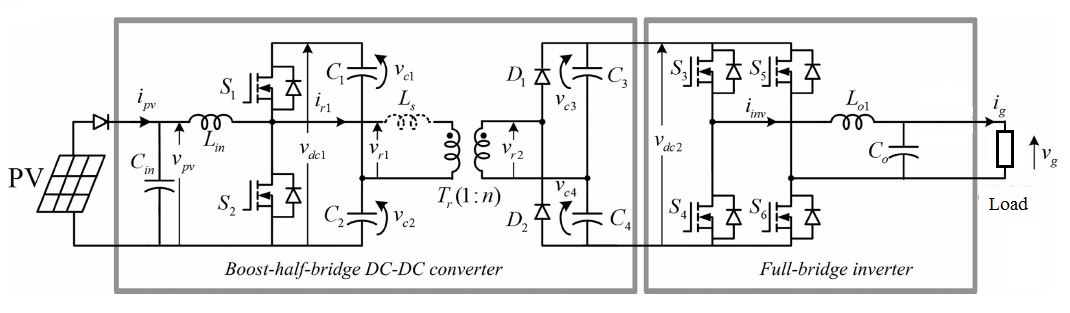
\includegraphics[width= 14 cm]{ct.jpg}
% \caption{ System Circuit Diagram}
% \end{figure}


% \section{Motivation for this work}

% There are  . . .

\section{Methodologies}

  Several three-dimensional models were constructed according to our test
  matrix, using the commercial, computational fluid dynamics package ANSYS FLUENT.The construction was carried out with the preprocessor of the package ANSYS WORKBENCH.Then the models were transferred to the processor FLUENT for executing the simulation. Finally, the post processor of the package FLUENT RESULT was used to study, analyze, and manipulate the results.
  
  The details of the modeling will be discussed in the next chapter. In the fourth chapter we provided the corroboration with the theoretical and historical results and a more extensive fin examination of the observations. In the fifth chapter the results of the simulations of the tested configurations are discussed. The final chapter draws certain conclusions and provides some recommendations.
\\  
  Because fins are used to improve heat transfer, it is important to allow open spaces toward optimization. In other words, the shape of fins must be optimized such that the heat transfer density is maximized when the space and the materials used for the finned surfaces are constraints



% \section{Outline of the Report}

% This report contains 6 chapters. Chapter 1 gives the introduction to   the project work and describes the objectives of the work. Literature    survey is describes in Chapter 2. An introduction to the pro............


\chapter{PROBLEM DESCRIPTION}

\section{Project background}
Fins are surfaces that extend from an object to increase the rate of heat transfer to or from the environment by increasing convection. The amount of conduction, convection, or radiation of an object determines the amount of heat it transfers. Because fins are used to improve heat transfer, it is important to allow open spaces toward optimization. In other words, the shape of fins must be optimized such that the heat transfer density is maximized when the space and the materials used for the finned surfaces are constraints. Fins are most commonly used in heat exchanging devices such as radiators in cars, computer CPU heat sinks, and heat exchangers in power plants. They are also used in newer technology such as hydrogen fuel cells. Nature has also taken advantage of the phenomena of fins. The ears of jackrabbits and fennec foxes act as fins to release heat from the blood that flows through them.
Some typical fin configurations,

\begin{figure}[h]
	 \label{ss}    %Figure Label is used
	 \centering
	 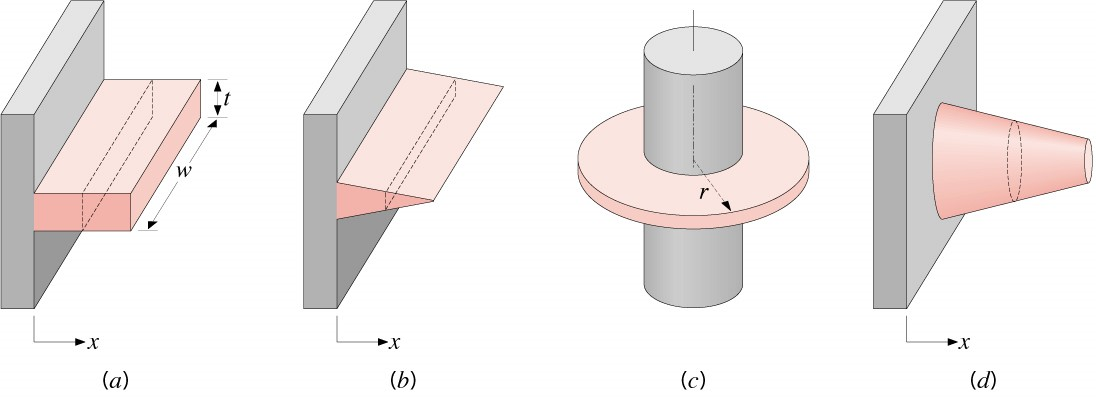
\includegraphics[width= 14 cm]{101.jpg}
	 \caption{ Fin Configurations}
	  \end{figure}
	  
	  Straight fins of (a) uniform and (b) non-uniform cross sections; (c) annular fin, and (d) pin fin of non-uniform cross section.
	  
	  
\section{Objective}

 The main objective of this study is to determine the performance and characteristics of flow and heat transfer behavior of plate fin of specific configurations. A 3-D model will be developed and whose behavior is examined for different hole diameters on the fin for a laminar compressible flow regime.
 
 The parameters that will be inspected are the, the heat
 transfer coefficient, the base temperature, the velocity profile, the temperature profile ,and the optimum hole diameter .The theoretical definitions for the above parameters will be provided in the following chapter. The results will be used to define suitable regions-conditions of operation for every fin geometry and to deduce the optimum optimum heat transfer value. 
 The base temperature and Effective heat transfer coefficient is calculated in the following cases
 
  \begin{itemize}
  \item{Plate fin having three 5mm holes}
  \item{Plate fin having three 10mm holes  }
  \item{Plate fin having three 15mm holes}
  \item{Plate fin having three 20mm holes  }
 \item{Plate fin having three 23mm holes  }
 \item{Plate fin having three variable holes 10,15,20 mm holes  }
 \end{itemize}
	
 \section{Scope}
 
 Fins are most commonly used in heat exchanging devices such as radiators in cars, computer CPU heatsinks, and heat exchangers in power plants.They are also used in newer technology such as hydrogen fuel cells.Nature has also taken advantage of the phenomena of fins.The ears of jackrabbits and fennec foxes act as fins to release heat from the blood that flows through them.

%Here you write abt the details in the IEEE paper(Intro + Conclusion) or about the work who had done before, what are the problems at that time, etc


%To use bullets

% \begin{itemize}
% \item{Presented}
% \item{Paper  }
% \item{Presented}
% \item{Paper  }
% \end{itemize}

% General, a micro-inverter PV \index{Photovoltaic} is often provided by a low voltage solar panel, which requires a high voltage lift ratio to produce the desired AC output .

% To use cascaded bullets

% \begin{itemize}
% \item{Presented}
% \item{Paper  }
%	\begin{itemize}
%		\item{Presented}
%		\item{Paper  }
%	\end{itemize}
% \item{Presented}
% \item{Paper  }
% \end{itemize}


%Inverter has become a future trend for single phase photovoltaic (PV) power. In general, a micro-inverter PV \index{Photovoltaic} is often provided by a low voltage solar panel . . . \vspace{2 cm} % Vspace to leave 2 cm space

% To use 1,2,3, numbers

% \begin{enumerate}
% \item prepare a source file with the extension "tex"
% \item Compile it with \LaTeX to produce a "dvi" file
% \item Print the document using a "dvi" driver
% \end{enumerate}


%  For making a table . .. .

% \begin{table}[h]
% \centering
% \begin{tabular}{|l|r|}  % use c for center alignment
% \hline
% Planet & Diameter(km)\\
% \hline
% Mercury & 4878\\
% Pluto & 2274\\
% Mercury & 4878\\
% Pluto & 2274\\
% Mercury & 4878\\
% Pluto & 2274\\
% Mercury & 4878\\
% Pluto & 2274\\
% \hline
% \end{tabular}
% \caption{Table Name}
% \end{table}



\chapter{GOVERNING EQUATION}  % Short of the project name

%  {\em Give some intro abt this chapter . . .. .  . }


\section{Basic fin equations}


\begin{figure}[h]
	\label{ss}    %Figure Label is used
	\centering
	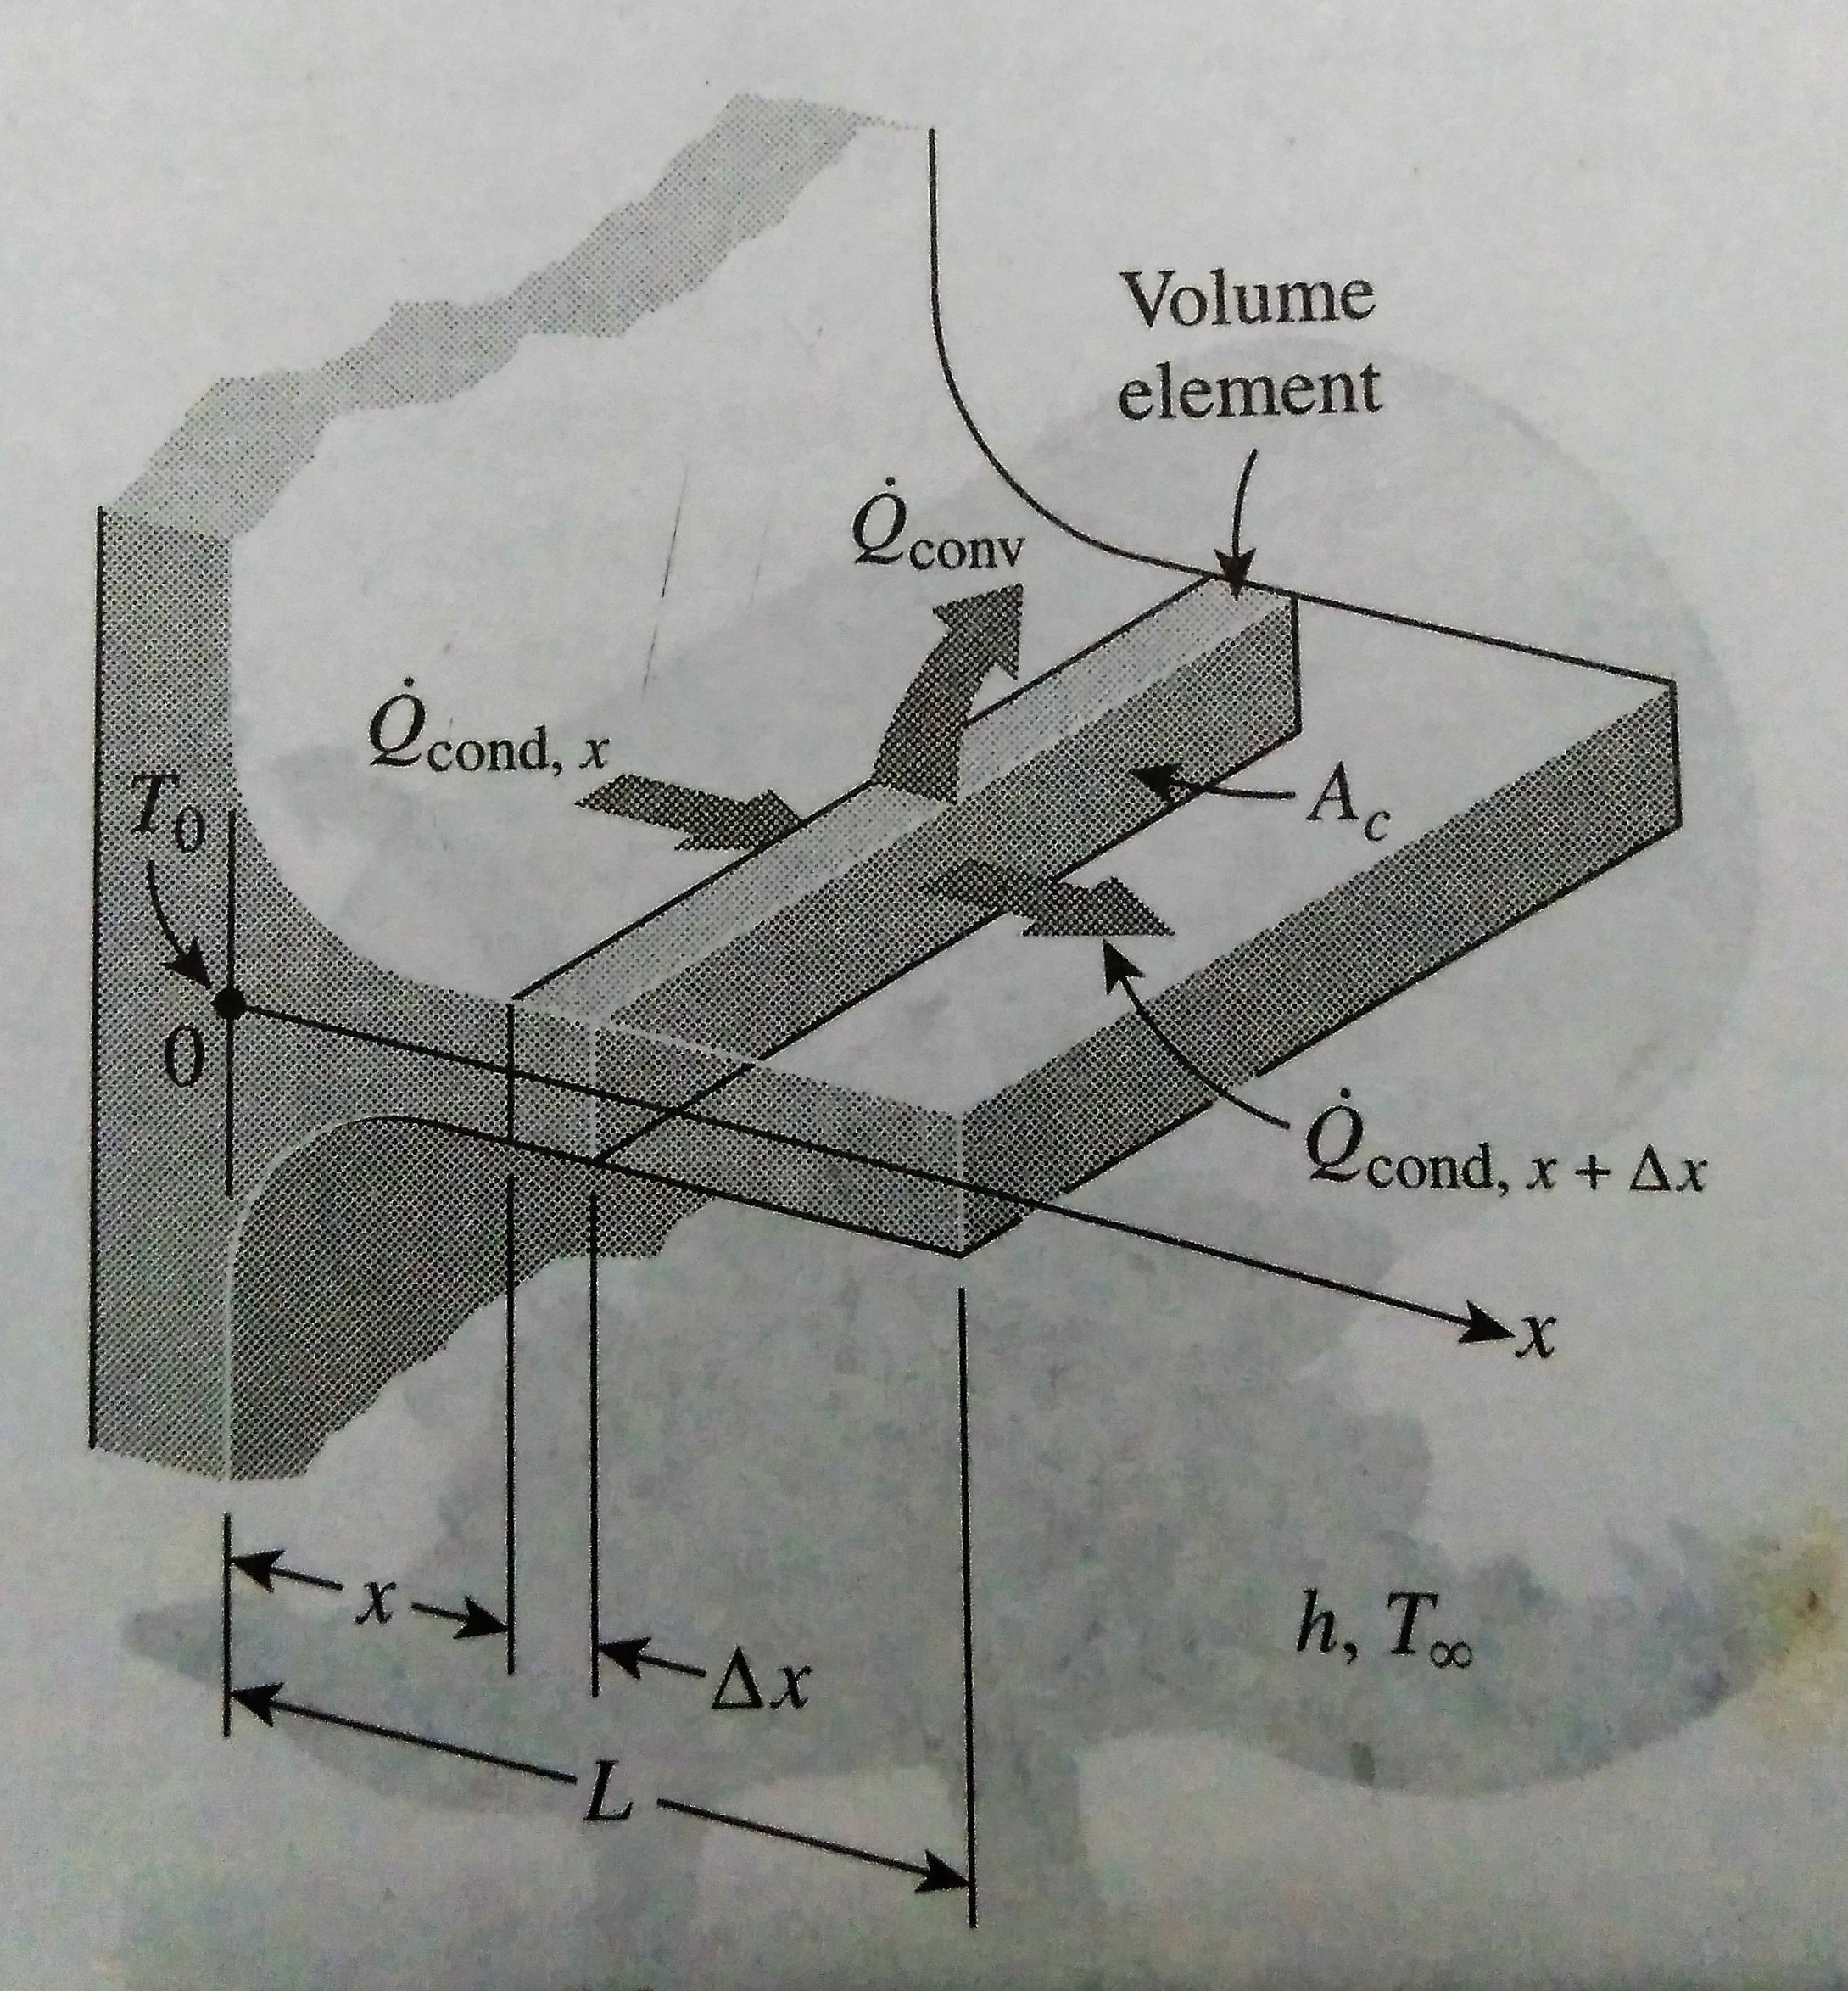
\includegraphics[width= 6 cm]{102.jpg}
	\caption{ Volume Element Of Fin }
\end{figure}


Consider a volume element of a fin at location $x$ having a length $ \Delta x $, cross sectional area of $ A_c $, and a perimeter of $ p $ ,as shown in figure. Under steady conditions, the energy balance on the volume element can be expressed as 

\begin{equation}
\dot{Q}_{cond,x}= \dot{Q}_{cond,x + \Delta x} + \dot{Q}_{conv}
\end{equation}  

where

\begin{equation}
    \dot{Q}_{conv} = h(p \Delta x)(T - T_\infty)
\end{equation}  

substituting and dividing by $ \Delta x $ ,we obtain

\begin{equation}
\frac{\dot{Q}_{cond,x + \Delta x}-\dot{Q}_{cond,x} }{\Delta x} + h p (T - T_\infty)= 0
\end{equation}  

Taking the limit as $ \Delta x  \rightarrow 0 $gives

\begin{equation}
\frac{\dot{Q}_{cond,x} }{\partial x} + h p (T - T_\infty)= 0
\end{equation} 

From Fouriers law of heat conduction we have 

\begin{equation}
\dot{Q}_{cond}= -k A_c \dfrac{dT}{dx}
\end{equation} 

Where $ A_c$, is the cross-sectional area of the fin at location $x$ . Substitution of this relation into 3.4 gives the differential equation governing heat transfer in fins,

\begin{equation}
\frac{d}{dx}(k A_c \frac{dT}{dx}) - hp(T-T_\infty) = 0
\end{equation} 

In general, the cross-sectional area $A_c$ and the perimeter $p$ of a fin vary with x, which makes this differential equation difficult to solve. In the special case of constant cross section and constant thermal conductivity, the differential equation 3.6 reduces to
\begin{equation}
\frac{d^2 T}{d x^2} - \frac{hp}{kA_c}(T-T_\infty) = 0
\end{equation}

or

\begin{equation}
\frac{d^2 \varTheta}{d x^2} - m^2 \varTheta = 0
\end{equation}

where $m^2 = hp / kA_c$  \\
and $ T-T_\infty $ is the temperature excess
 
\section{Governing Differential Equation }

The individual differential equation that we shall encounter express a certain conservation principle. Each equation employs a certain physical quantity as it's dependent variable and implies that there must be a balance among the various factors that influence the variable. The dependent variables of these differential equations are usually specific properties, ie quantities expressed on a unit mass basis.Examples are mass fraction, velocity(momentum per unit mass) and specific enthalpy.

\subsection{Energy equation}

The energy equation in its most general form contains a large number of influences.Since we are primarily interested in the form rather than in the details of the equation, it will be sufficient to consider some restricted cases.
\\
For a stedy low-velocity flow with negligible viscous dissipation, the energy equation can be written as 

\begin{equation}
div(\rho uh)=div(k \ grad \ T) + S_h
\end{equation}  

where $h$ is the specific enthalpy, $k$ is the thermal conductivity, $T$ is the temperature, and $S_h$ is the volumetric rate of heat generation. The term $div(k grad T)$ represents the influence of conduction heat transfer within the fluid.According to Fourier's law of conduction.
\\
For ideal and for solids and liquids, we can write
 \begin{equation}
 c \ grad  \ T = grad \ h
 \end{equation}  
 
 where $c$ is the constant-pressure specific heat. With this substitution, the energy equation becomes
 \begin{equation}
 div(\rho uh)=div(\frac{k}{c} grad T) + S_h
 \end{equation}  
 
 If $c$ is constant, the $ h~T $ relation simplifies to
 \begin{equation}
 h=cT
 \end{equation}  
 which would lead to
 \begin{equation}
 div(\rho uT)=div(\dfrac{k}{c} \ grad \ T) + \dfrac{S_h}{c}
 \end{equation}  
 In this manner, either the enthalpy or the temperature can be chosen as the dependent variablee.
 \\
 The steady heat conduction situation is obtained by setting velocity $u = 0$ thus
 \begin{equation}
 div(k \ grad \ T) + S_h = 0
 \end{equation}  

 
 \subsection{Momentum Equation}
 
 The differential equation governing the conservation of momentum in a given direction for a Newtonian fluid can be written along similar lines ; however, the complication is greater because both shear and normal stresses must be considered and because the Stokes viscosity law is more complicated than Fick's law or Fourier's law. With $u$ denoting the x-direction velocity, we write the corresponding momentum equation as 
 
 \begin{equation}
 \dfrac{\partial}{\partial t}(\rho u) + div(\rho u \textbf{u}) =  div(\mu \ grad \ u) - \dfrac{\partial p}{\partial x} + B_x + V_x
 \end{equation}  
 
 where $\mu$ is the viscosity, $p$ is the pressure, $B_x$ is the x direction body force per unit volume, and $V_x$ stands for the viscous term that are in addition to those expressed by $div(\mu \ grad u)$
 
 \subsection{Conservation Of Mass}
 
 Law of conservation of mass states that total mass will be conserved in a system. Rate of increase of mass will be equal to Net influx of mass in the system.
  \begin{equation} 
  \frac{\partial}{\partial t}\int_V \rho dv = - \oint_s \rho \textbf{u}.\textbf{n} ds 
  \end{equation}
 
 \chapter{NUMERICAL ANALYSIS}
 
 
 
 
 


\section{Grid Independence Study}

Convergence is something that all CFD engineers talk about, but we must remember that the way we generally define convergence is only a small part of ensuring that we have a valid solution. For a steady state simulation we need to endure that the solution satisfies the following three conditions:
\begin{itemize}
	\item 	Residual RMS error values have reduced to an acceptable value ( typically 10-4 or 10-5 )
	\item Monitor points for our values of interest have reached a steady solution.
\item The domain has imbalance of less than 1\%.
\end{itemize}
Our values of interest are essentially the main outputs from our simulation, so pressure drop, forces, mass flow etc. we need to make sure that these have converged to a steady value otherwise if we let the simulation run for an additional 50 iterations then the result will be different. Ensuring that these values have reached a steady solution means that we are basing our decisions on a single repeatable value.
As a rule we must ensure that prior to starting a simulation we clearly define what our values of interest are, and we make sure that we monitor these to ensure that they reach a steady state. As previously highlighted, we also need to make sure that the residual RMS error values are to at least 10-4. Finally, we need to ensure that the overall imbalance in the domain is less than 1% for all variables.
The approach outlined above results in a single solution for the given mesh that we have used. Although we are happy that this has ‘converged’ based on the RMS error values, monitor points and imbalance, we need to make sure that the solution is also independent of the mesh resolution. Not checking this is a common cause of erroneous results in CFD, and this process should at least be carried out once for each type of problem that we deal with so that the next time a similar problem arises, we can apply the same mesh sizing.
The best way to check for a mesh independent solution is to plot a graph of the resultant monitor value vs the number of cells in the simulation. In this simulation the resultant monitor value is the temperature. We plot a graph with temperature in y-axis and number of mesh elements in x-axis.


\begin{figure}[h]
	\label{ss}    %Figure Label is used
	\centering
	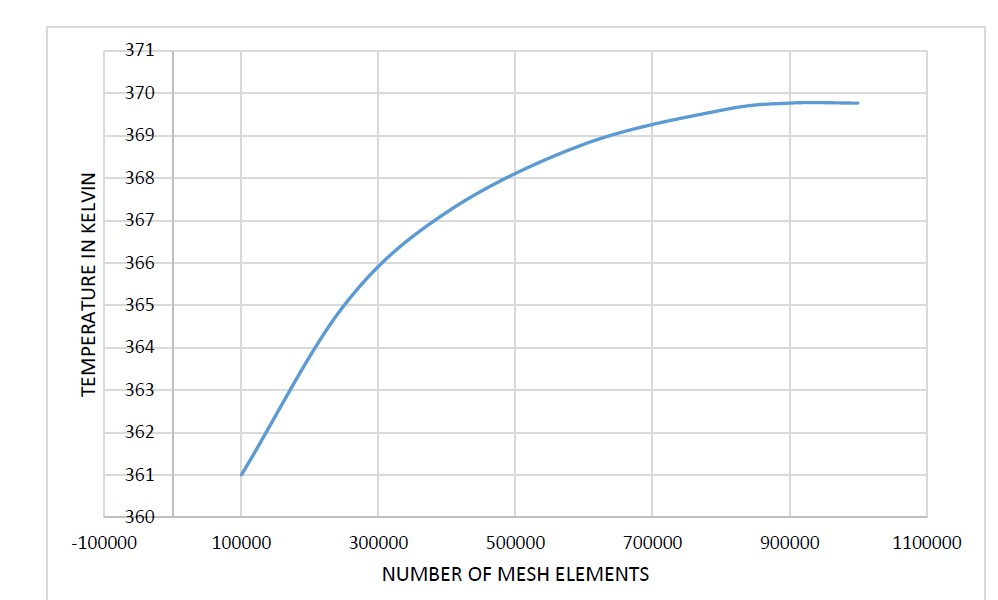
\includegraphics[width= 10 cm]{103.jpg}
	\caption{ Grid Independent Study}
\end{figure}

We can see that with 3 lakh cells we have a result, which could be converged for that particular mesh, with 10-4 residuals and imbalance below 1\%. By increasing the mesh resolution to 9 lakh cells, we can see that there has been a jump in the value of interest.
By increasing the mesh size further we can see that the 11 lakh cell simulation results in a value that is within the acceptable range. This indicates that we have reached a solution that is independent of the mesh resolution, and for further analysis we can use the 9 lakh cell case, as it will give us a result within the use defined tolerance. 


\section{Plate Fin Base Line Study}

		In the study of heat transfer, fin are surfaces that extend from an object to increase the rate of heat transfer to or from the environment by increasing convection. The amount of conduction, convection or radiation of an object determines the amount of heat it transfers. Increasing the temperature gradient between the object and the environment, increasing the convection heat transfer coefficient, or increasing the surface area of the object increases the heat transfer. Sometimes it is not feasible or economical to change the first two options. Thus, adding a fin to an object , increases the surface area and can sometimes be an economical solution to heat transfer problems. 
		
\subsection{Modelling}

The numerical modelling was performed using the ANSYS DESIGN MODELER of the commercial finite element analysis package ANSYS. 


\begin{figure}[h]
	\label{ss}    %Figure Label is used
	\centering
	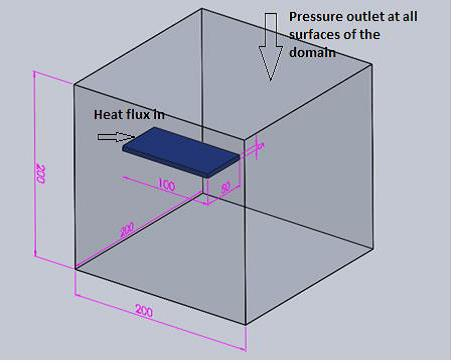
\includegraphics[width= 10 cm]{104.jpg}
	\caption{ Grid Independent Study}
\end{figure}

In this experiment we used rectangular fin. The fin type is selected as solid.
And the geometric parameters of the fin are; \\
Length			=     100mm \\
Breadth 		=      50mm \\
Thickness		=       5mm \\
This rectangular fin is confined in an air domain. Air is selected as the fluid medium so as to increase the computational accuracy.  The geometry of the air domain is cube with side 200mm in length.

\subsection{Solution Technique}
\subsubsection{Flow Approximations}
\begin{itemize}
	\item  \textbf{Inviscid flow}
	When two fluid layer s move relative to each other, a friction force develops between them and the slower layer tries to slow down the faster layer. This internal resistance to flow is quantified by the fluid property viscosity, which is a measure of internal stickiness of the fluid. Viscosity is caused by cohesive forces between the molecules in liquids and by molecular collision in gases. There is no fluid with zero viscosity, and thus all fluid flows involve viscous effect to some degree. Flows in which the frictional effects are significant are called viscous flows. However, in many flows of practical interests, there are regions (typically regions not close to solid surfaces) where viscous forces are negligibly small compared to inertial or pressure forces. Neglecting the viscous terms in such inviscid flow regions greatly simplifies the analysis without much loss in accuracy.   
	
	\item \textbf{Incompressible flow}
	A flow is classified as being compressible or in compressible depending on the level of variation of density during flow. A flow is said to be in compressible if the density remains constant throughout. Therefore, the volume of every portion of fluid remains unchanged over the course of its motion when the flow is incompressible.
	Liquid flows are incompressible to a high level of accuracy, but the level of variation in density in gas flows and the consequent level of approximation made when modeling gas flows as incompressible depends on the Mach number defined as M = V / c , where c is the velocity of sound whose value is 346 m/s in air at room temperature at sea level. Gas flows can often be approximated as incompressible if the density changes are under about 5 percent, which is usually the case when Ma < 0.3. Therefore, the compressibility effects of air can be neglected at speeds under about 100 m/s. That means flow of gas is not necessarily a compressible flow.
	
	\item \textbf{ Laminar flow}
	Some flows are smooth and orderly while the others are rather chaotic. The highly ordered fluid motion characterized by smooth layers of fluid is called laminar. The flow of high-viscosity fluids such as oils at low velocity is typically laminar. The highly disordered fluid motion that typically occurs at high velocities and is characterized by velocity fluctuations is called turbulent. Since the air velocity is negligible in this case we assume it as a laminar flow regime.
	
	\item \textbf{Natural convection}
	A fluid flow is said to be natural or forced, depending on how the fluid motion is initiated. In forced flow, a fluid is forced to flow over a surface or in a pipe by external means such as a pump or a fan. In natural flows, any fluid motion is due to natural means such as the buoyancy effect, which manifests itself as the rise of the warmer (and thus lighter) fluid and the fall of cooler (and thus denser) fluid.
	
	\item  \textbf{Steady flow}
	A steady flow implies a flow pattern in which flow properties do not change with time. It refers to flow that has reached its final equilibrium state. During steady flow, the fluid properties can change from pont to point within a device, but at any fixed point they remain constant.           
	
\end{itemize}
\subsubsection{The Boussinesq Approximation }
In fluid dynamics, the Boussinesq approximation is used in the field of buoyancy-driven flow (also known as natural convection). It ignores density differences except where they appear in terms multiplied by g, the acceleration due to gravity. The essence of the Boussinesq approximation is that the difference in inertia is negligible but gravity is sufficiently strong to make the specific weight appreciably different between the two fluids.
Boussinesq flows are common in nature (such as atmospheric fronts, oceanic circulation, katabatic winds), industry (dense gas dispersion, fume cupboard ventilation), and the built environment (natural ventilation, central heating). The approximation is extremely accurate for many such flows, and makes the mathematics and physics simpler.
\\
The Boussinesq approximation is applied to problems where the fluid varies in temperature from one place to another, driving a flow of fluid and heat transfer. The fluid satisfies conservation of mass, conservation of momentum and conservation of energy. In the Boussinesq approximation, variations in fluid properties other than density   are ignored, and density only appears when it is multiplied by  , the gravitational acceleration.
\\
\textbf{Advantages}
\\
The approximation's advantage arises because when considering a flow of, say, warm and cold water of density $ \rho_1 $ and $ \rho_2 $  one needs only to consider a single density $ \rho$ : the difference $\Delta\rho = \rho_1 - \rho_2 $  is negligible. Dimensional analysis shows that, under these circumstances, the only sensible way that acceleration due to gravity g should enter into the equations of motion is in the reduced gravity   where
	
	
\subsection{Boundary Condition}




To solve the equation system, we also need boundary conditions. The typical boundary conditions in CFD are no-slip boundary condition, axisymmetric boundary condition, inlet, outlet boundary condition and periodic boundary condition.
For example, in a pipe, the fluid flows from left to right. We can use inlet at left side, which means we can set the velocity manually. At the right side, we use outlet boundary condition to keep all the properties constant, which means all the gradients are zero. At the wall of pipe, we can set the velocity to zero. This is no-slip boundary condition. At the center of pipe, we can use axisymmetric boundary condition.

Almost every computational fluid dynamics problem is defined under the limits of initial and boundary conditions. For implementation of boundary conditions when we construct a staggered grid we add an extra node across the physical boundary in order to get,	
\begin{itemize}
	\item •	The nodes just outside the inlet of the system are used to assign the inlet conditions
	\item •	The physical boundaries can coincide with the scalar control volume boundaries.
\end{itemize}

This allow us to introduce the boundary conditions and achieve discretion equations for nodes near boundary with small modifications.
\\

Most common boundary conditions used in computational fluid dynamics are
\begin{itemize}
	\item Intake conditions
	\item Symmetry conditions
	\item Physical boundary conditions
	\item Cyclic conditions
	\item pressure conditions
	\item exit conditions
\end{itemize}



\textbf{Boundary Conditions Used In Experiment}

\begin{itemize}
	\item Heat flux in to the fin is given at the base of the fin. Heat flux =  24000 $W/m^2$
\item	Operating temperature around the fin is considered as 300 $K$
\item	Pressure outside the domain is considered as atmospheric ( 101325 $Pa$)
\item	The analysis is conducted on a rectangular aluminium fin having
\\ 
\ Thermal conductivity = 202 $ W/mK $
\\
\ Density 		= 2719 $kg/m^3$
\\
\ Specific heat		= 871 $J/kg \ K$

\item	The working fluid is air having
\\
\ Density		= 1.165 $ kg/m^3$
\\
\ Dynamic viscosity	= 1.84 $ \times  10^{-5}  Ns/m^2 $
\\
\ Specific heat		= 1005 $J/kg \ K$
\\
\ Thermal conductivity	= 0.025 $W/mK$
\\
\ Thermal expansion coefficient = 0.0033 $ oC^{-1}$

\end{itemize}







\section{Meshing}

In computational solutions of partial differential equations, meshing is a discrete representation of the geometry that is involved in the problem. Essentially, it partitions space into elements (or cells or zones) over which the equations can be approximated.

\subsection{Mesh Quality}

The mesh quality can be conclusively determined based on the following factors.Higher mesh quality ensures better results.
\\

\textbf{Rate of convergence}
\\
The greater the rate of convergence, the better the mesh quality. It means that the correct solution has been achieved faster. An inferior mesh quality may leave out certain important phenomena such as the boundary layer that occurs in fluid flow. In this case the solution may not converge or the rate of convergence will be impaired.
\\
\textbf{Solution accuracy}
\\
A better mesh quality provides a more accurate solution. For example, one can refine the mesh at certain areas of the geometry where the gradients are high, thus increasing the fidelity of solutions in the region. Also, this means that if a mesh is not sufficiently refined then the accuracy of the solution is more limited. Thus, mesh quality is dictated by the required accuracy.
\\
\textbf{CPU time required}
\\
CPU time is a necessary yet undesirable factor. For a highly refined mesh, where the number of cells per unit area is maximum, the CPU time required will be relatively large. Time will generally be proportional to the number of elements.
\\

\subsection{Grid Classification}

\subsubsection{Structured grids}

Structured grids are identified by regular connectivity. The possible element choices are quadrilateral in 2D and hexahedra in 3D. This model is highly space efficient, i.e. since the neighborhood relationships are defined by storage arrangement. Some other advantages of structured grid over unstructured are better convergence and higher resolution

\subsubsection{Unstructured grids}

An unstructured grid is identified by irregular connectivity. It cannot easily be expressed as a two-dimensional or three-dimensional array in computer memory. This allows for any possible element that a solver might be able to use. Compared to structured meshes, this model can be highly space inefficient since it calls for explicit storage of neighborhood relationships. These grids typically employ triangles in 2D and tetrahedra in 3D. 

\subsubsection{Hybrid grids}

A hybrid grid contains a mixture of structured portions and unstructured portions. It integrates the structured meshes and the unstructured meshes in an efficient manner. Those parts of the geometry that are regular can have structured grids and those that are complex can have unstructured grids. These grids can be non-conformal which means that grid lines don’t need to match at block boundaries.


\begin{figure}[h]
        \centering
        \begin{subfigure}[b]{0.3\textwidth}
                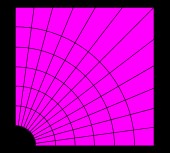
\includegraphics[width=\textwidth]{105.jpg}
                \caption{Structured}
                \label{fig:structured}
        \end{subfigure}%
        ~ %add desired spacing between images, e. g. ~, \quad, \qquad, \hfill etc.
          %(or a blank line to force the subfigure onto a new line)
        \begin{subfigure}[b]{0.3\textwidth}
                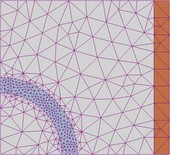
\includegraphics[width=\textwidth]{106.jpg}
                \caption{Unstructured}
                \label{fig:unstructured}
        \end{subfigure}
        ~ %add desired spacing between images, e. g. ~, \quad, \qquad, \hfill etc.
          %(or a blank line to force the subfigure onto a new line)

        \caption{Mesh Types}\label{fig:Meshing}
\end{figure}

\textbf{Meshing used}
\\
\underline{Hexahedron}


 A hexahedron, a topological cube, has 8 vertices, 12 edges, bounded by 6 quadrilateral faces. It is also called a hex or a brick. For the same cell amount, the accuracy of solutions in hexahedral meshes is the highest.
The pyramid and triangular prism zones can be considered computationally as degenerate hexahedrons, where some edges have been reduced to zero. Other degenate forms of a hexahedron may also be represented.

\subsection{Mesh Properties}

\subsubsection{Skewness}

The skewness of a grid is an apt indicator of the mesh quality and suitability. Large skewness compromises the accuracy of the interpolated regions. There are three methods of determining the skewness of a grid.

\subsubsection{Aspect ratio}

It is the ratio of longest to the shortest side in a cell. Ideally it should be equal to 1 to ensure best results. For multidimensional flow, it should be near to one. Also local variations in cell size should be minimal, i.e. adjacent cell sizes should not vary by more than 20 \%. Having a large aspect ratio can result in an interpolation error of unacceptable magnitude.



\begin{figure}[h]
	\label{ss}    %Figure Label is used
	\centering
	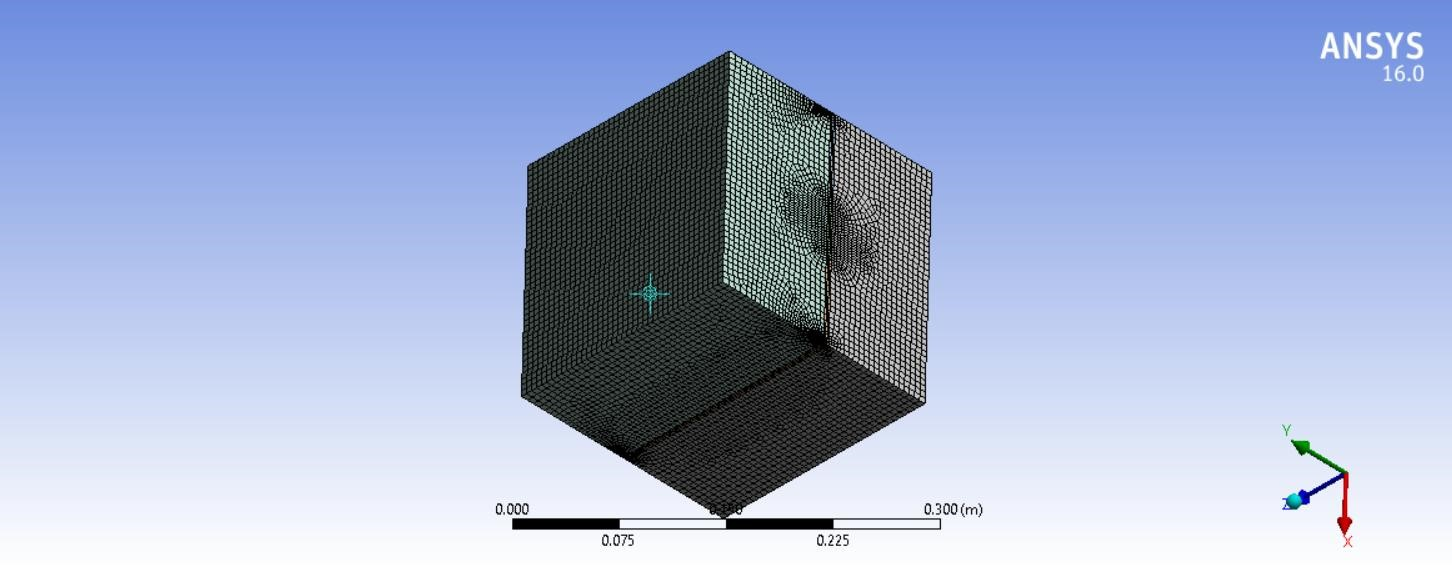
\includegraphics[width= 15 cm]{107.jpg}
	\caption{ Meshing}
\end{figure}





\section{Data Reduction}


\subsection{CFD Analysis}
Computational fluid dynamics (CFD) study of the system starts with the construction of
desired geometry and mesh for modeling the dominion. Generally, geometry is simplified
for the CFD studies. Meshing is the discretization of the domain into small volumes
where the equations are solved by the help of iterative methods. Modeling starts with the
describing of the boundary and initial conditions for the dominion and leads to modeling
of the entire system. Finally, it is followed by the analysis of the results, conclusions and
discussions.
In CFD calculations, there are three
main steps.
\begin{itemize}
	\item  Pre-Processing
 \item Solver Execution
\item  Post-Processing
\end{itemize}
Pre-Processing is the step where the
modeling goals are determined and
computational grid is created. In the second
step numerical models and boundary
conditions are set to start up the solver.
Solver runs until the convergence is reached.
When solver is terminated, the results are
examined which is the post processing part.
\subsection{Solution}

1.\textbf{Problem Setup}
\\
The mesh is checked and quality is obtained. The analysis type is changed
to Pressure Based type. The velocity formulation is changed to absolute and
time to steady state. Gravity is defined as y = -9.81 $m/s^2$
\\
2.\textbf{Models}
\\
Energy is set to ON position. Viscous model is selected as laminar.
\\
3.\textbf{Materials}
\\
Material are selected , aluminum is chosen for the fin and air for the domain.We also chose density variation to follow the boussniq approximation.
\\
4.\textbf{Cell Zone Conditions}
\\
The parts are assigned as air and aluminum as per fluid/solid parts.
\\
5.\textbf{Boundary conditions}
\\
The fin base is selected as a wall and given a thermal heat flux of 24000 $W / m^2 $.Also the air domain outer surface is given as pressure outlet having zero gauge pressure (atmospheric pressure).

\subsection{Temperature Plot}

The temperature of the fin will vary along the length. This variation is shown in figure 4.5 .The plot is made on the top surface of the fin along its length having coordinates $p_1 = (.1 , .1 , 0)$ and $ p_2 = (.1 , .1 , .1) $,units are in meter.
 
\begin{figure}[h]
	\label{ss}    %Figure Label is used
	\centering
	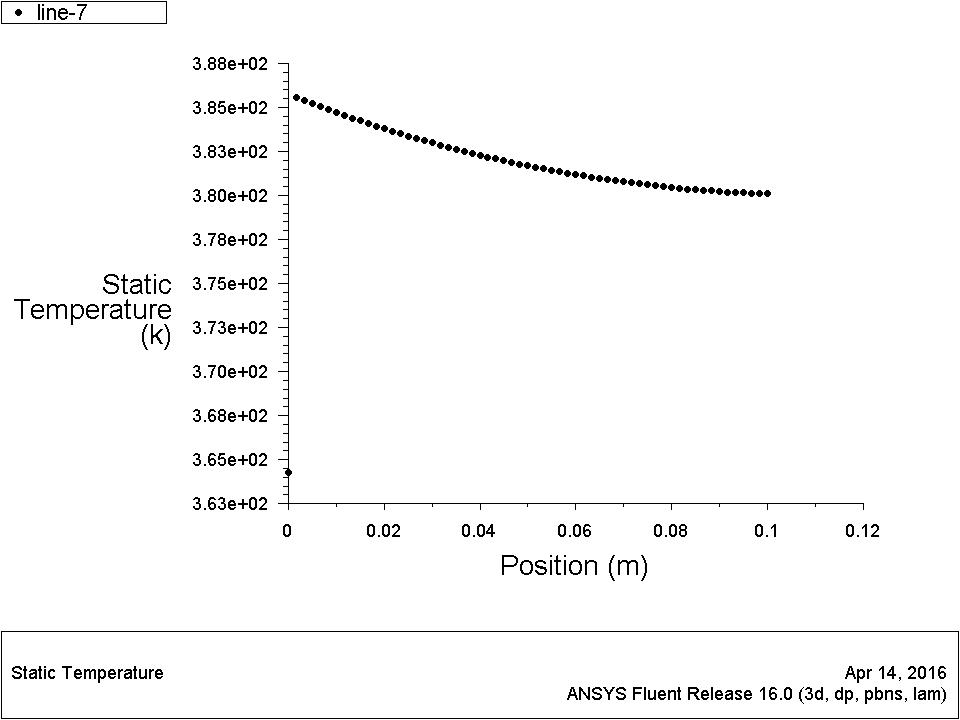
\includegraphics[width= 10 cm]{108.jpg}
	\caption{ Temperature variation along lenth of fin}
\end{figure}


\subsection{Heat transfer coefficient plot}

The heat transfer coefficient also varies along the length and is shown in fig 4.6. The plot is made on the top surface of the fin along its length having coordinates $p_1 = (.1 , .1 , 0)$ and $p_2 = (.1 , .1 , .1) $,units are in meter.

\begin{figure}[h]
	\label{ss}    %Figure Label is used
	\centering
	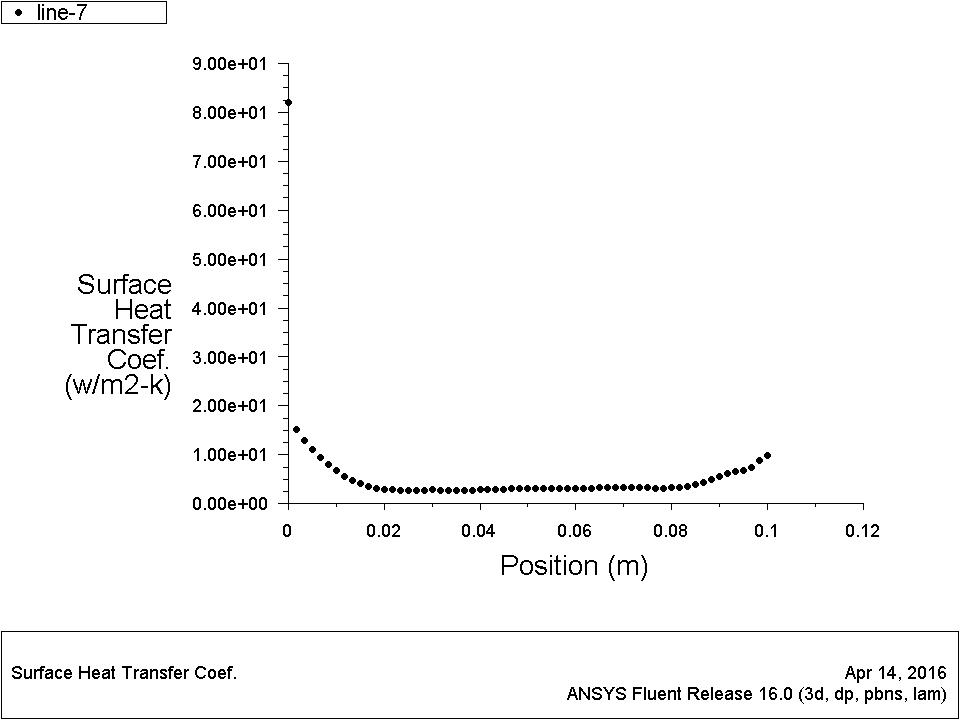
\includegraphics[width= 10 cm]{109.jpg}
	\caption{ h variation along lenth of fin}
\end{figure}

\section{Result And Discussion}

\subsection{Base temperature}

The temperature at the base of the fin depends on the amount of heat liberated through the fin surface. 

$ T_b = 385.802 K $


\subsection{ Effective heat transfer Coefficient}

We know heat transfer in a fin is through by both conduction and convection. We recognize that the convective heat transfer coefficient $h$, in general varies along the fin length as well as its circumference, and its value at a point is a strong function of the fluid motion at that point. The value of h is usually much lower at the fin base than it is at the fin tip because the fluid is surrounded by solid surfaces near the base, which seriously disrupt its motion to the point of “suffocating” it, while the fluid near the fin tip has little contact with a solid surface and thus encounters little resistance to flow.

So for analysis of fin we define a average / effective heat transfer coefficient. This heat transfer coefficient value depend on base temperature and ambient temperature
\begin{equation}
h_{eff} =  \frac{Q}{A \ (T_b - T_\infty)}
\end{equation} 


For the plate fin


\begin{equation}
h_{eff} =  \frac{24000}{11250 \ (385.802 - 300)}
\end{equation} 


$ h_{eff} $ =  2.79 $W / m^2 K $

\subsection{Contours}

\subsubsection{Temperature Contour}

The figure 4.7 shows the temperature contour of a plate cutting the fin cross-sectionally having co-ordinates $ p_1 = (.1,0,0) , p_2 = (.1,0,.2) $ and $ p_3 = (.1,.2,.2) $


\begin{figure}[h]
\label{ss}    %Figure Label is used
\centering
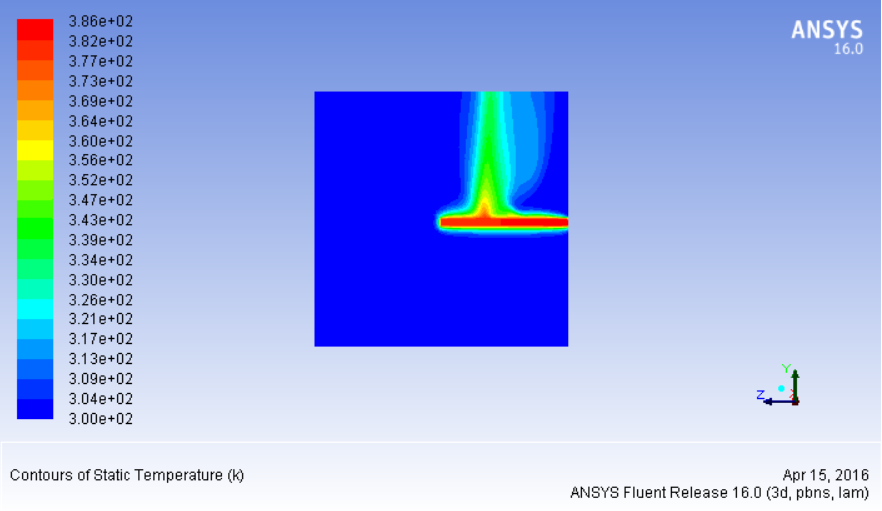
\includegraphics[width= 11 cm]{110.png}
\caption{Temperature Contour}
\end{figure}

\subsubsection{Velocity Contour}

The figure 4.8 shows the velocity contour of a plate cutting the fin cross-sectionally having co-ordinates $ p_1 = (.1,0,0) , p_2 = (.1,0,.2) $ and $ p_3 = (.1,.2,.2) $


\begin{figure}[h]
	\label{ss}    %Figure Label is used
	\centering
	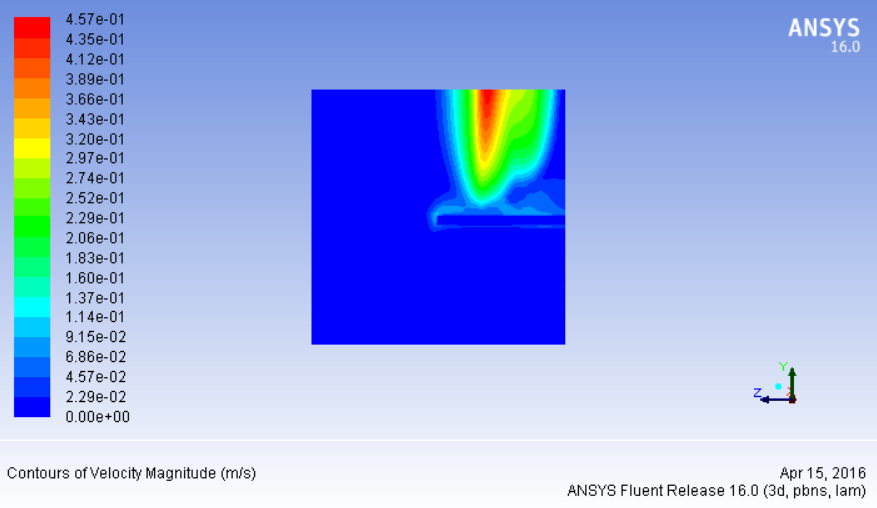
\includegraphics[width= 11 cm]{111.png}
	\caption{Velocity Contour}
\end{figure}


\subsubsection{Velocity Vector Contour}

The figure 4.9 shows the Velocity vector of a plate cutting the fin cross-sectionally having co-ordinates $ p_1 = (.1,0,0) , p_2 = (.1,0,.2) $ and $ p_3 = (.1,.2,.2) $


\begin{figure}[h]
	\label{ss}    %Figure Label is used
	\centering
	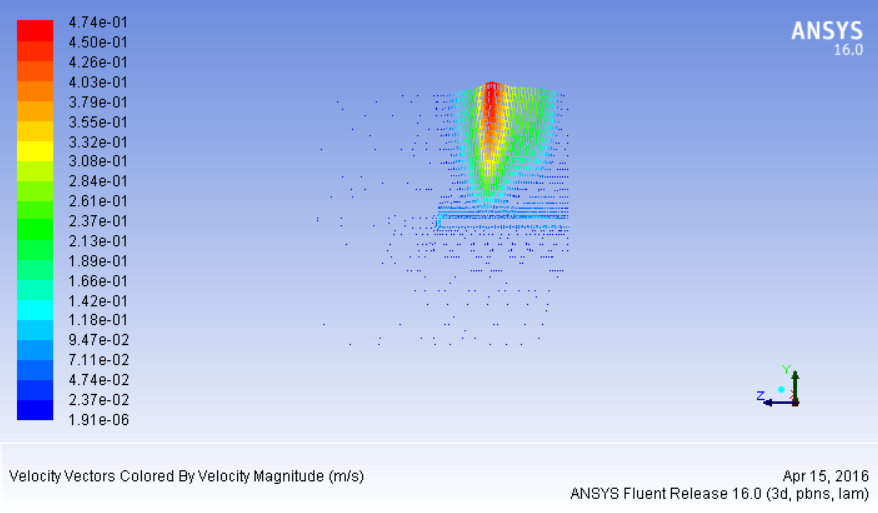
\includegraphics[width= 11 cm]{112.png}
	\caption{Velocity Vector}
\end{figure}









\chapter{EFFECT OF HOLES ON PLATE FIN}

\section{Modelling}

Three equidistant holes were put on the fin surface. The diameter of hole was then increased and its effect on heat transfer rate was studied. 

\begin{figure}[h]
	\label{ss}    %Figure Label is used
	\centering
	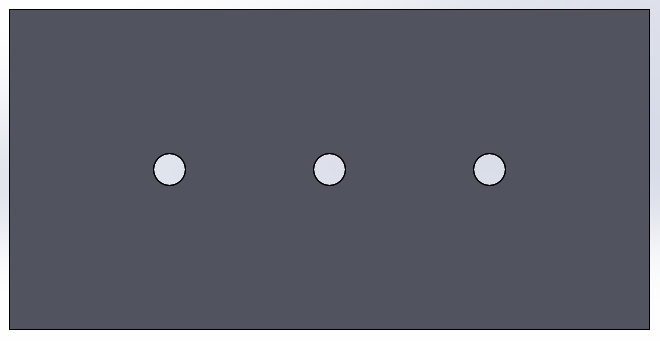
\includegraphics[width= 11 cm]{113.png}
	\caption{Holes of 5mm dia on bottom}
\end{figure}

\begin{figure}[h]
	\label{ss}    %Figure Label is used
	\centering
	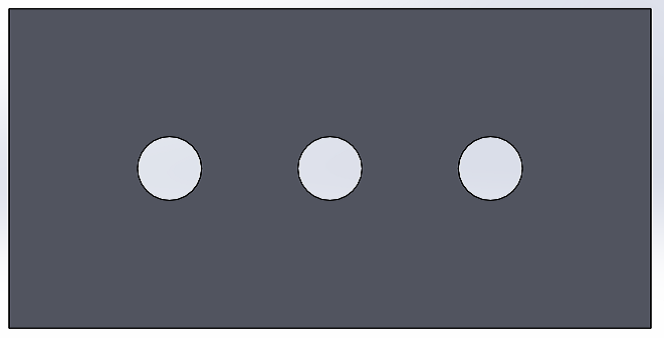
\includegraphics[width= 11 cm]{114.png}
	\caption{Holes of 10mm dia on bottom}
\end{figure}

\begin{figure}[h]
	\label{ss}    %Figure Label is used
	\centering
	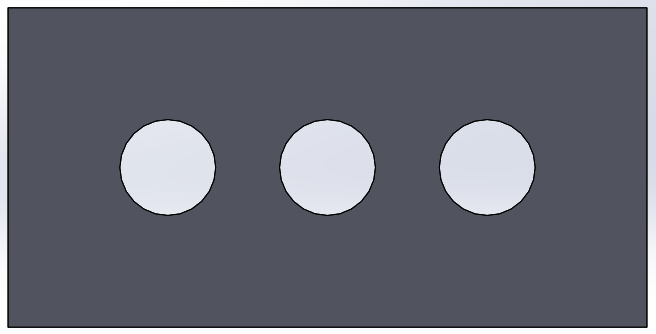
\includegraphics[width= 11 cm]{115.png}
	\caption{Holes of 15mm dia on bottom}
\end{figure}

\begin{figure}[h]
	\label{ss}    %Figure Label is used
	\centering
	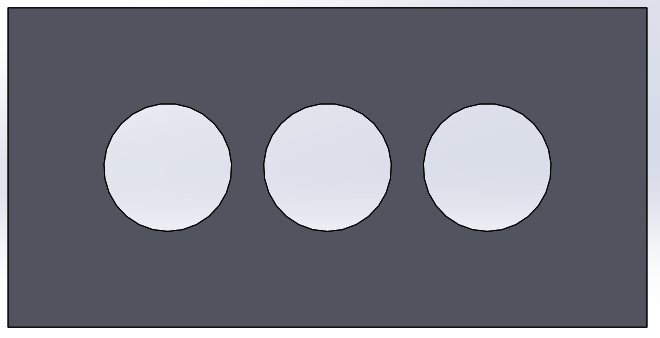
\includegraphics[width= 11 cm]{116.png}
	\caption{Holes of 20mm dia on bottom}
\end{figure}

\begin{figure}[h]
	\label{ss}    %Figure Label is used
	\centering
	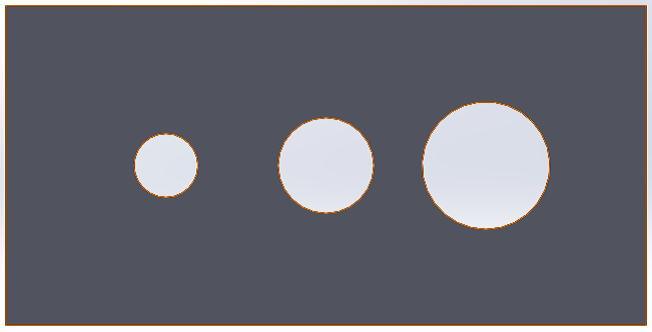
\includegraphics[width= 11 cm]{117.png}
	\caption{Holes of 10,15,20 mm dia on bottom}
\end{figure}

\section{Solution Technique}

The test model of this study consist of seven different configurations. The different configurations are based on the diameter of the circular hole on the surface of rectangular fin. This rectangular fin is analysed using CFD – FLUENT software.  All of the configurations have the same length, thickness and cross sectional area. First is a plane rectangular fin, second one is rectangular fin with 5mm hole diameter. Third one is a rectangular fin with 10 mm hole diameter. Fourth one is a rectangular fin with 15mm hole diameter. Fifth one is a rectangular fin with 20mm hole diameter. Sixth one is a rectangular fin with 23 mm hole diameter. Last one is a rectangular fin with varying hole diameter from base of the fin to the free end.

For every configurations we are providing the same heat flux (24000 W/m2).But based on the heat dissipation along the fin base temperature may vary for different configurations. The value of base temperature is found from FLUENT result files by using area weighted average method. 



\chapter{RESULT AND DISCUSSION}

Here we discuss selected performance characteristics of the rectangular fins that were analyzed. The characteristics are chosen to highlight various features of the behavior of fins for different hole diameters.

 \begin{figure}[h]
 	\centering
 	\begin{subfigure}[b]{0.5\textwidth}
 		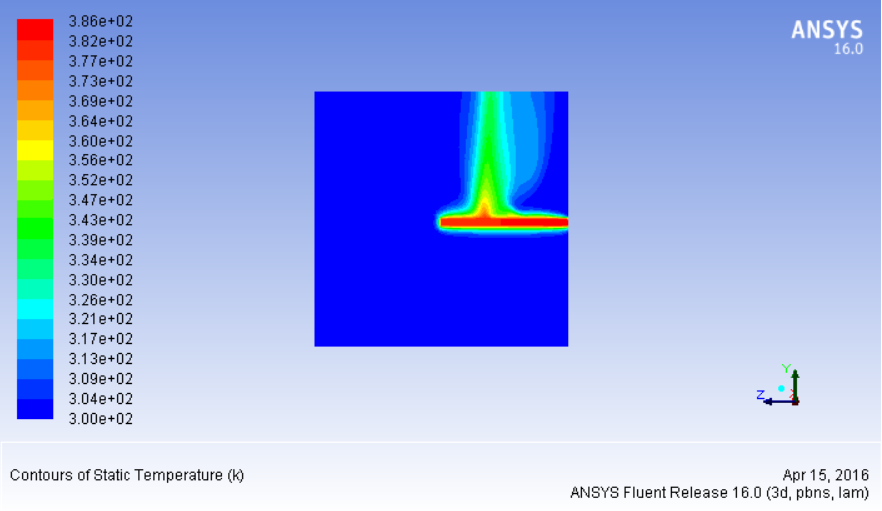
\includegraphics[width=\textwidth]{110.png}
 		\caption{plane fin}
 		\label{fig:structured}
 	\end{subfigure}%
 	
 	\begin{subfigure}[b]{0.5\textwidth}
 		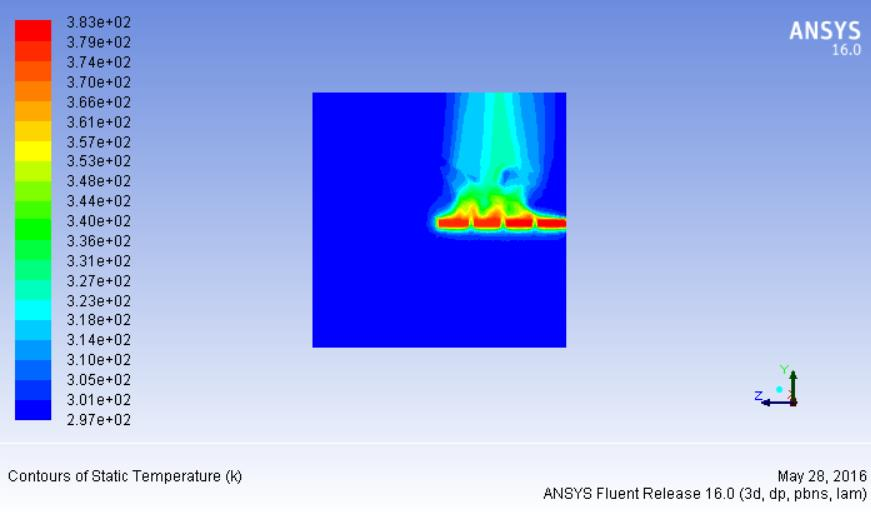
\includegraphics[width=\textwidth]{121.jpg}
 		\caption{5mm hole}
 		\label{fig:structured}
 	\end{subfigure}%
 	~ %add desired spacing between images, e. g. ~, \quad, \qquad, \hfill etc.
 	%(or a blank line to force the subfigure onto a new line)
 	\begin{subfigure}[b]{0.5\textwidth}
 		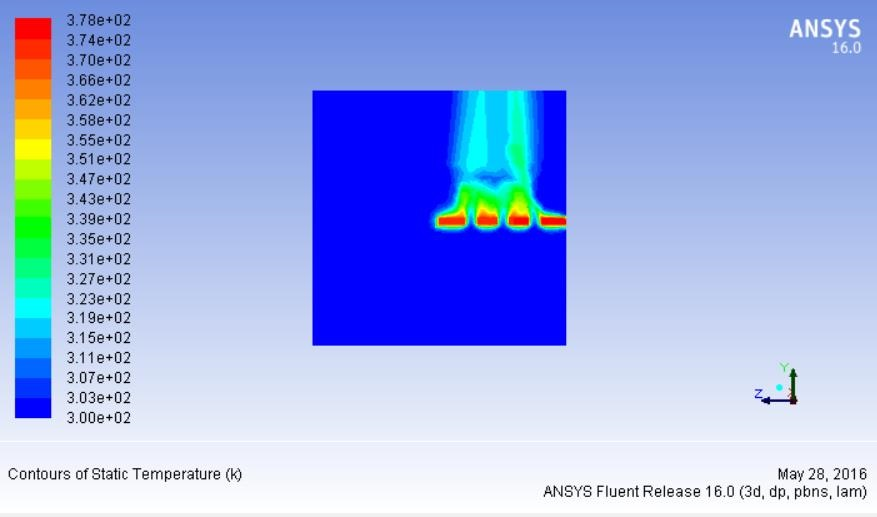
\includegraphics[width=\textwidth]{1211.jpg}
 		\caption{10 mm fin}
 		\label{fig:unstructured}
 	\end{subfigure}
 	~ %add desired spacing between images, e. g. ~, \quad, \qquad, \hfill etc.
 	%(or a blank line to force the subfigure onto a new line)
 	\begin{subfigure}[b]{0.5\textwidth}
 		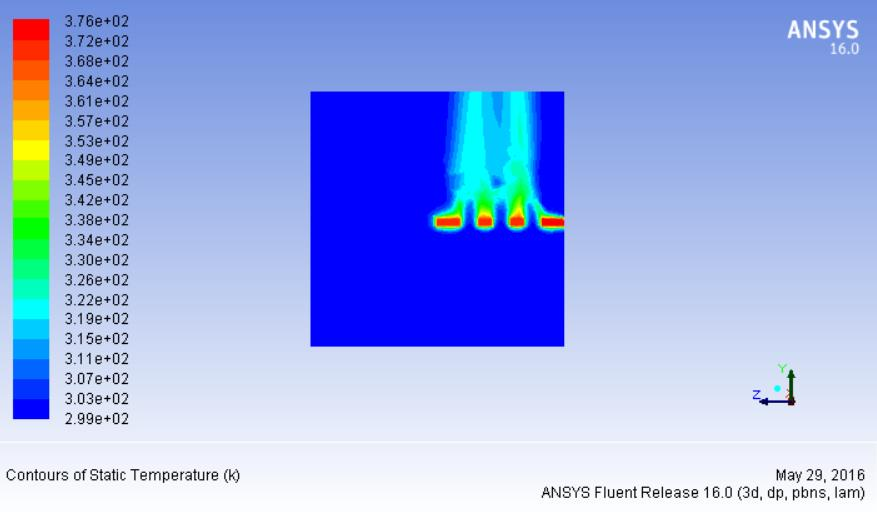
\includegraphics[width=\textwidth]{122.jpg}
 		\caption{15mm hole}
 		\label{fig:structured}
 	\end{subfigure}%
 	~ %add desired spacing between images, e. g. ~, \quad, \qquad, \hfill etc.
 	%(or a blank line to force the subfigure onto a new line)
 	\begin{subfigure}[b]{0.5\textwidth}
 		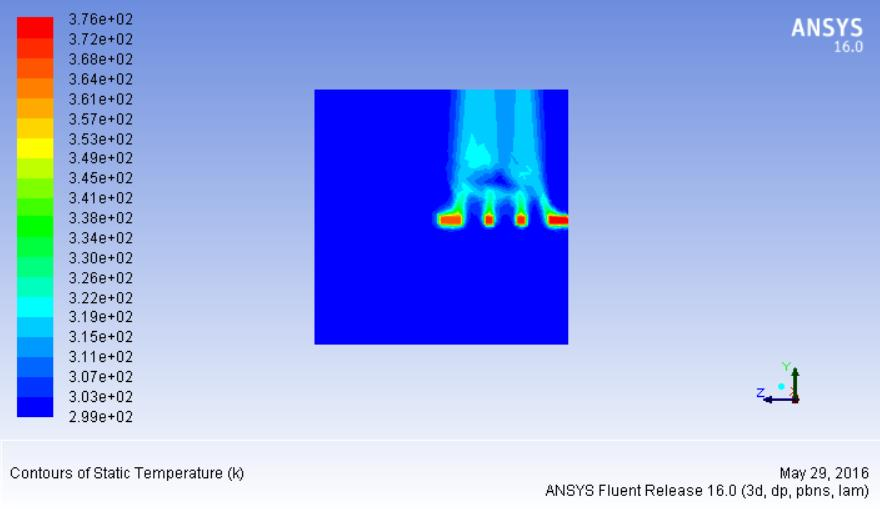
\includegraphics[width=\textwidth]{123.jpg}
 		\caption{20 mm hole}
 		\label{fig:unstructured}
 	\end{subfigure}
 	~ %add desired spacing between images, e. g. ~, \quad, \qquad, \hfill etc.
 	%(or a blank line to force the subfigure onto a new line)
 	\begin{subfigure}[b]{0.5\textwidth}
 		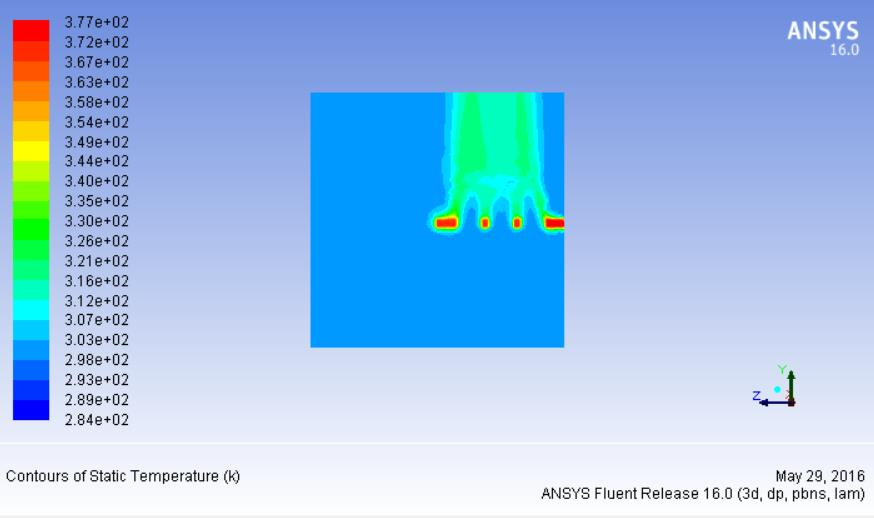
\includegraphics[width=\textwidth]{124.jpg}
 		\caption{23mm hole}
 		\label{fig:structured}
 	\end{subfigure}%
 	~ %add desired spacing between images, e. g. ~, \quad, \qquad, \hfill etc.
 	%(or a blank line to force the subfigure onto a new line)
 	\begin{subfigure}[b]{0.5\textwidth}
 		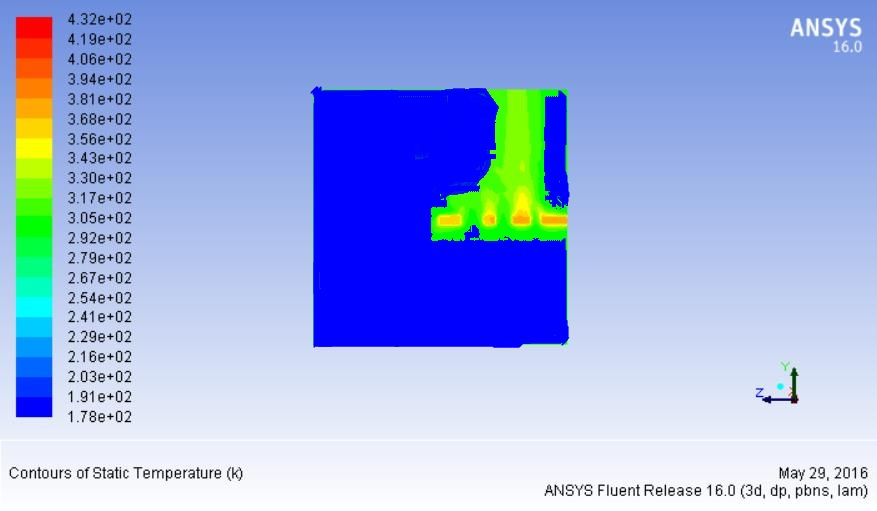
\includegraphics[width=\textwidth]{125.jpg}
 		\caption{variable hole}
 		\label{fig:unstructured}
 	\end{subfigure}
 	
 	~ %add desired spacing between images, e. g. ~, \quad, \qquad, \hfill etc.
 	%(or a blank line to force the subfigure onto a new line)
 	\caption{Temperature Contour }\label{fig:Meshing}
 \end{figure}



\section{Effect Of Radius}

                       The effect of radius is one of the most critical and interesting of the examined parameters.In order to compare the results we inspect the the changes in heat transfer coefficient for different hole diameter.
                       
                       We know heat transfer in a fin is through by both conduction and convection. We recognize that the convective heat transfer coefficient $h$, in general varies along the fin length as well as its circumference, and its value at a point is a strong function of the fluid motion at that point. The value of h is usually much lower at the fin base than it is at the fin tip because the fluid is surrounded by solid surfaces near the base, which seriously disrupt its motion to the point of “suffocating” it, while the fluid near the fin tip has little contact with a solid surface and thus encounters little resistance to flow.
                       On putting holes to the plate fin we observe that the hot air at the fin base can now rise through these holes instead of flowing through the circumference(figure velocity vector of plate fin).This fluid motion enhances heat transfer , since it brings warmer and cooler chunks of fluid into contact ,initiating higher rate of conduction at a greater number of sites in a fluid. Hence the rate of heat transfer through fluid is much higher. In fact, the higher the fluid velocity, the higher the rate of heat transfer.  

 \begin{figure}[h]
 	\centering
 	\begin{subfigure}[b]{0.5\textwidth}
 		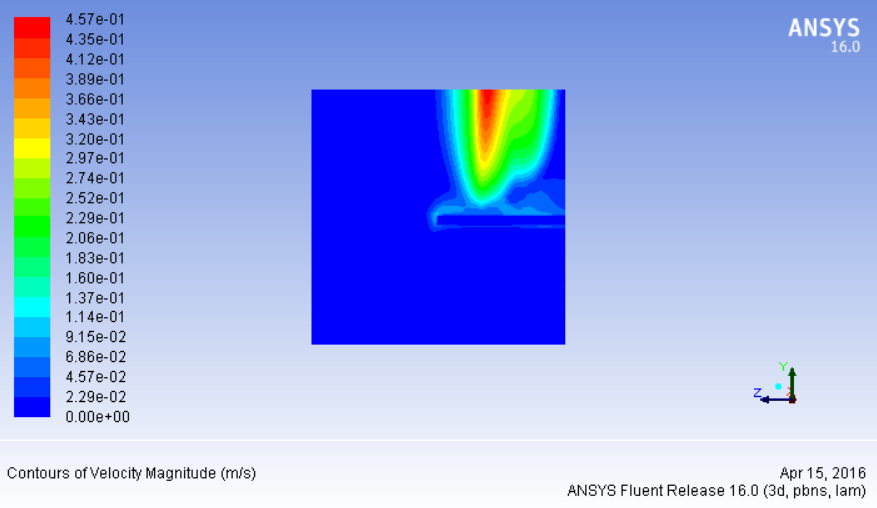
\includegraphics[width=\textwidth]{111.png}
 		\caption{plane fin}
 		\label{fig:structured}
 	\end{subfigure}%
 	
 	\begin{subfigure}[b]{0.5\textwidth}
 		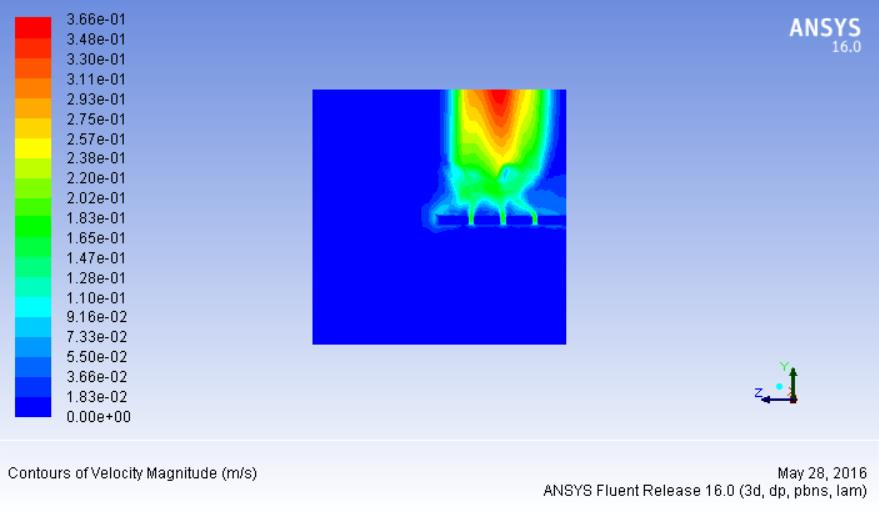
\includegraphics[width=\textwidth]{133.jpg}
 		\caption{5mm hole}
 		\label{fig:structured}
 	\end{subfigure}%
 	~ %add desired spacing between images, e. g. ~, \quad, \qquad, \hfill etc.
 	%(or a blank line to force the subfigure onto a new line)
 	\begin{subfigure}[b]{0.5\textwidth}
 		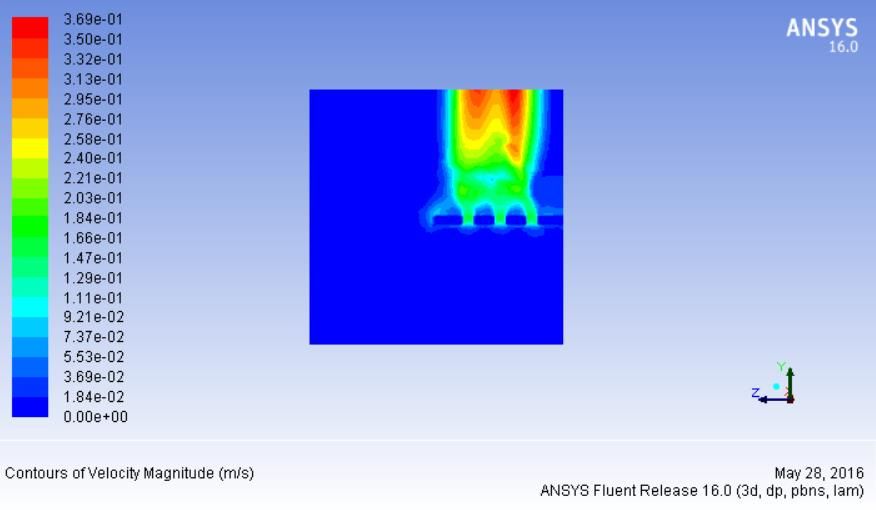
\includegraphics[width=\textwidth]{134.jpg}
 		\caption{10 mm fin}
 		\label{fig:unstructured}
 	\end{subfigure}
 	~ %add desired spacing between images, e. g. ~, \quad, \qquad, \hfill etc.
 	%(or a blank line to force the subfigure onto a new line)
 	\begin{subfigure}[b]{0.5\textwidth}
 		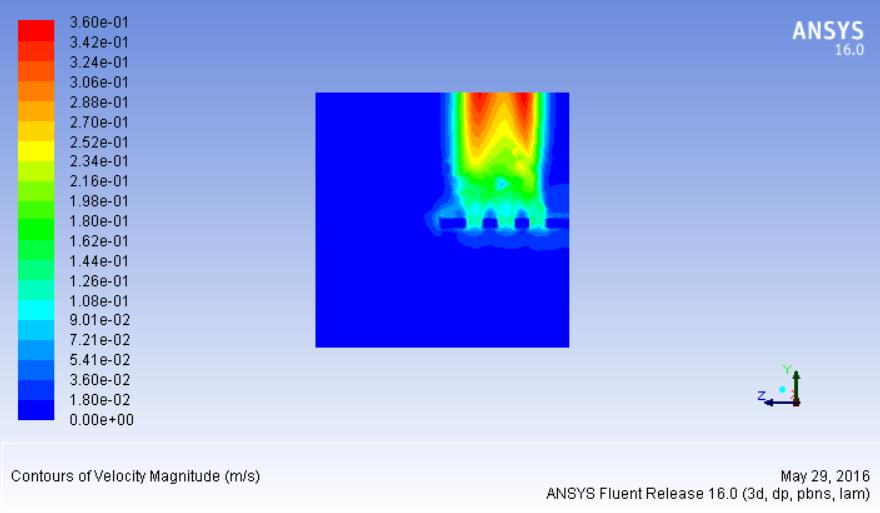
\includegraphics[width=\textwidth]{135.jpg}
 		\caption{15mm hole}
 		\label{fig:structured}
 	\end{subfigure}%
 	~ %add desired spacing between images, e. g. ~, \quad, \qquad, \hfill etc.
 	%(or a blank line to force the subfigure onto a new line)
 	\begin{subfigure}[b]{0.5\textwidth}
 		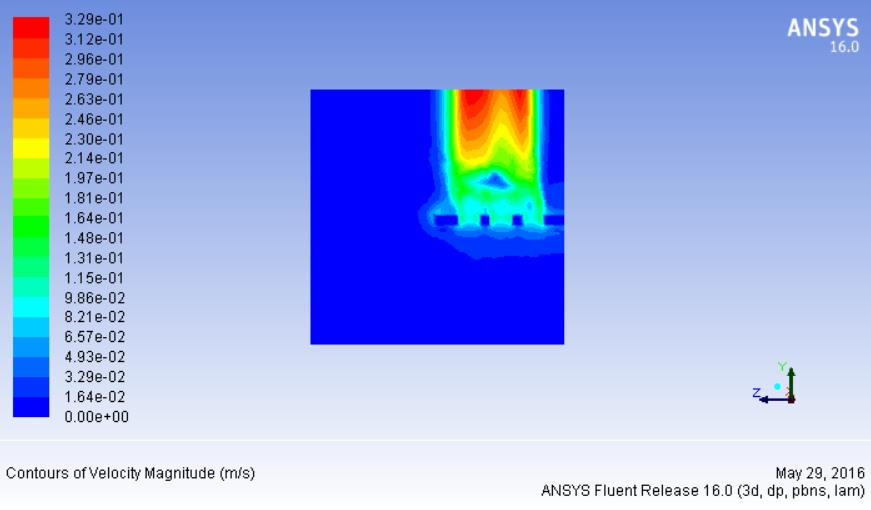
\includegraphics[width=\textwidth]{136.jpg}
 		\caption{20 mm hole}
 		\label{fig:unstructured}
 	\end{subfigure}
 	~ %add desired spacing between images, e. g. ~, \quad, \qquad, \hfill etc.
 	%(or a blank line to force the subfigure onto a new line)
 	\begin{subfigure}[b]{0.5\textwidth}
 		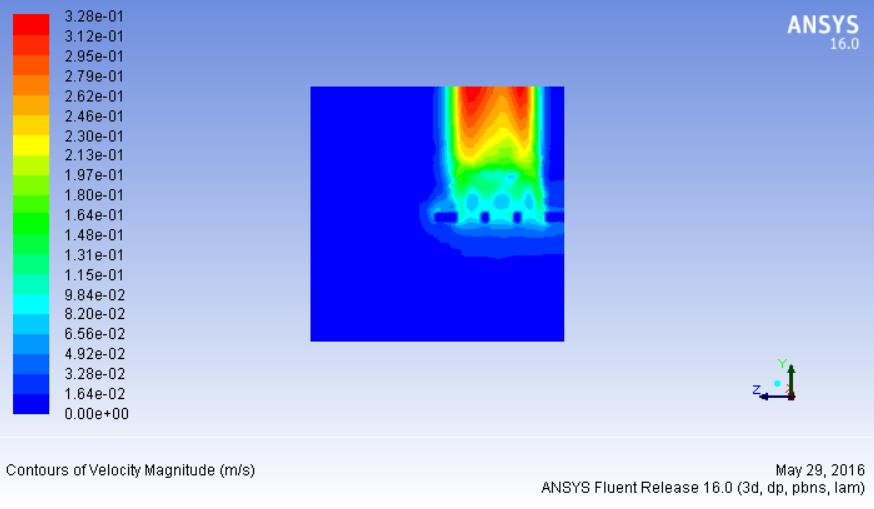
\includegraphics[width=\textwidth]{137.jpg}
 		\caption{23mm hole}
 		\label{fig:structured}
 	\end{subfigure}%
 	~ %add desired spacing between images, e. g. ~, \quad, \qquad, \hfill etc.
 	%(or a blank line to force the subfigure onto a new line)
 	\begin{subfigure}[b]{0.5\textwidth}
 		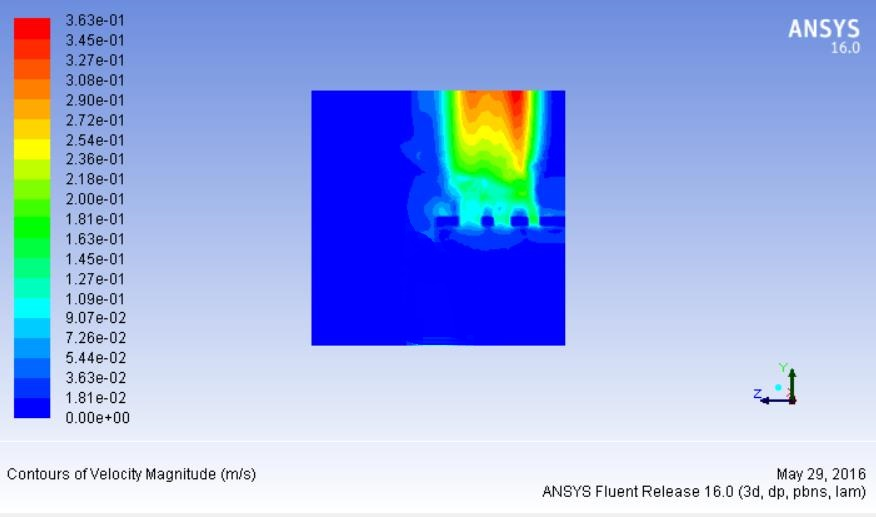
\includegraphics[width=\textwidth]{138.jpg}
 		\caption{variable hole}
 		\label{fig:unstructured}
 	\end{subfigure}
 	
 	~ %add desired spacing between images, e. g. ~, \quad, \qquad, \hfill etc.
 	%(or a blank line to force the subfigure onto a new line)
 	\caption{Velocity Contour }\label{fig:Meshing}
 \end{figure}


\section{Optimization}

	As we increase the hole diameter the fluid motion increases through this hole. Larger hole size means more room for surrounding air, more area available for convection. Thus convective heat transfer increases as we go on increasing the hole diameter. But after a particular limit the overall heat transfer decreases, this is because as we increase the hole size we are taking more material out from the fin. On decreasing the material content of the fin conduction through the fin decreases. The heat content at the base will not be completely transferred to the fin tip because of the reduced material. Therefore the overall heat transfer of the fin decreases. There is optimum value of heat transfer for a particular hole diameter value for which conduction and convection heat transfer balances each other. This can be found by repeating the analysis with larger diameter and finding the diameter at which the heat transfer decreases. This will be the optimum diameter for the given plate fin.
	It’s also interesting to note that conduction is predominant near the base and convection is predominant at the fin tip. We also know putting holes increases the convective heat transfer, so by putting larger holes near the tip and smaller holes near the base would enhance the overall heat transfer. This increase is depicted in figure 6.2


 \begin{figure}[h]
 	\centering
 	 	 	\begin{subfigure}[b]{0.5\textwidth}
 	 	 		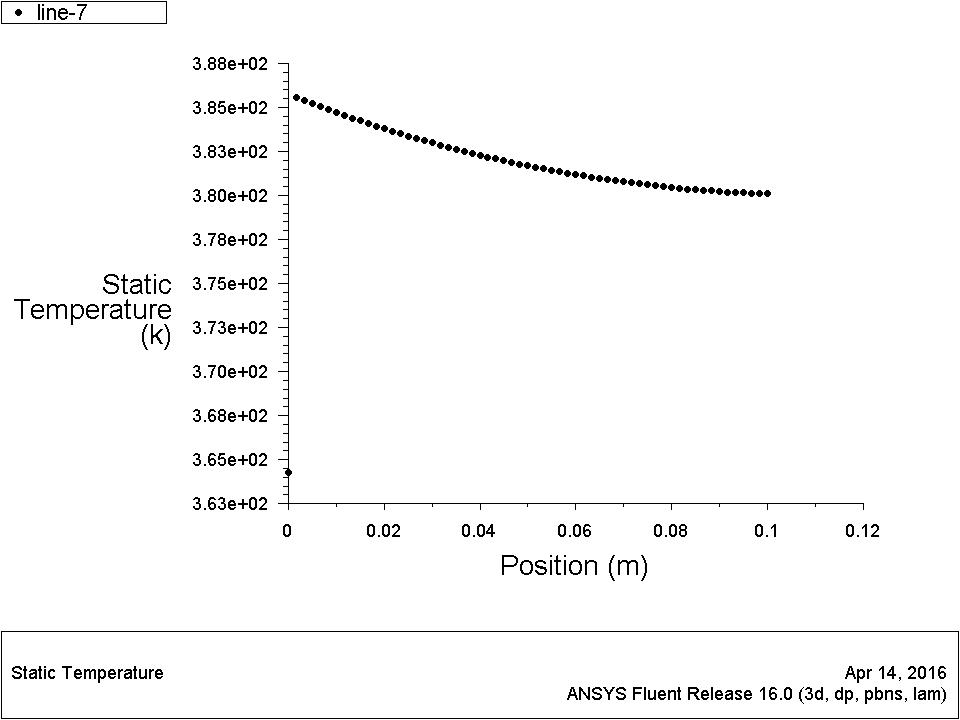
\includegraphics[width=\textwidth]{126.jpg}
 	 	 		\caption{plane fin}
 	 	 		\label{fig:structured}
 	 	 	\end{subfigure}%
 	 	 	
 	\begin{subfigure}[b]{0.5\textwidth}
 		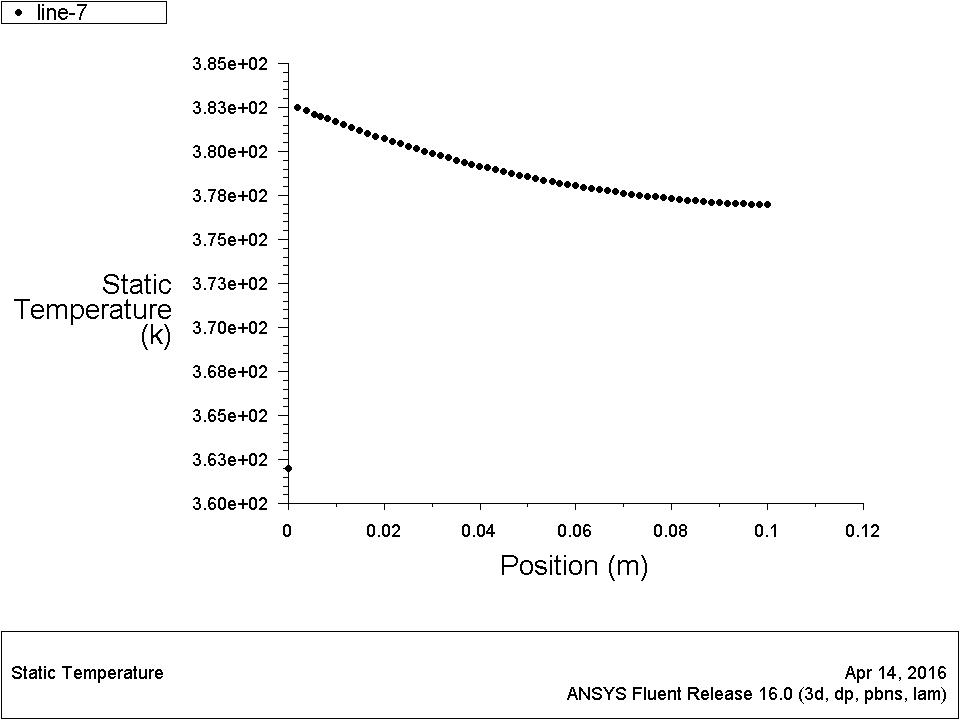
\includegraphics[width=\textwidth]{127.jpg}
 		\caption{5mm hole}
 		\label{fig:structured}
 	\end{subfigure}%
 	~ %add desired spacing between images, e. g. ~, \quad, \qquad, \hfill etc.
 	%(or a blank line to force the subfigure onto a new line)
 	\begin{subfigure}[b]{0.5\textwidth}
 		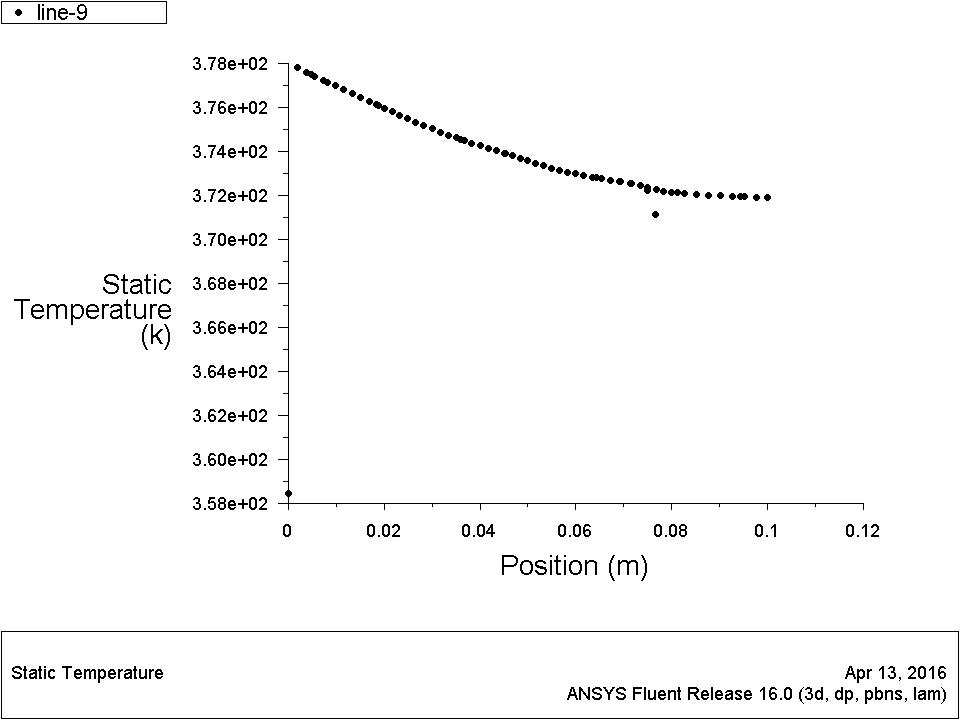
\includegraphics[width=\textwidth]{128.jpg}
 		\caption{10 mm fin}
 		\label{fig:unstructured}
 	\end{subfigure}
 	~ %add desired spacing between images, e. g. ~, \quad, \qquad, \hfill etc.
 	%(or a blank line to force the subfigure onto a new line)
 	\begin{subfigure}[b]{0.5\textwidth}
 		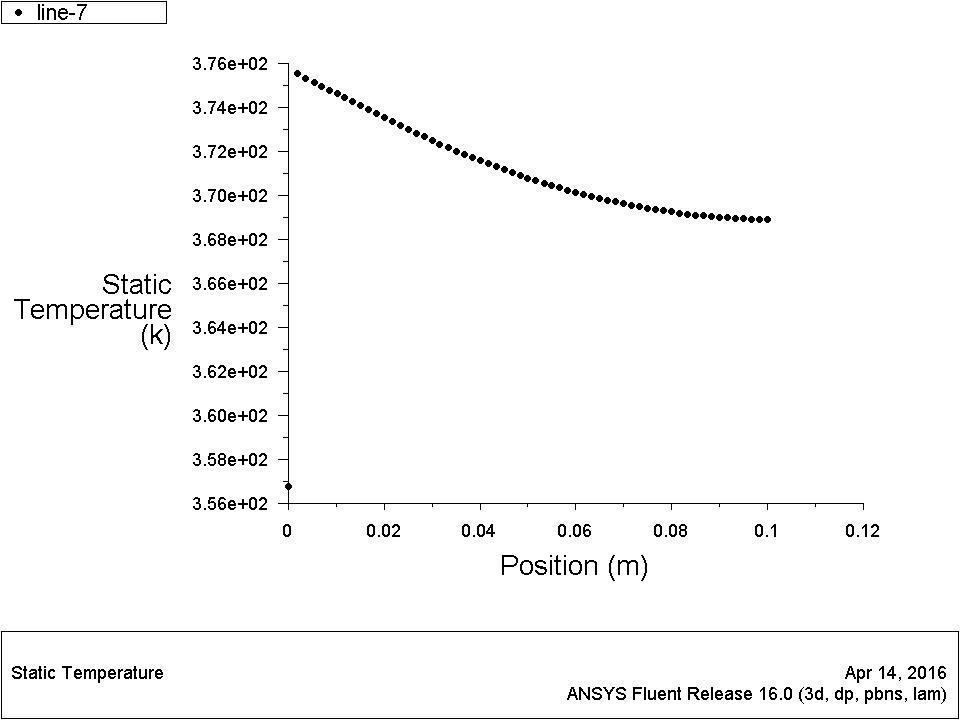
\includegraphics[width=\textwidth]{129.jpg}
 		\caption{15mm hole}
 		\label{fig:structured}
 	\end{subfigure}%
 	~ %add desired spacing between images, e. g. ~, \quad, \qquad, \hfill etc.
 	%(or a blank line to force the subfigure onto a new line)
 	\begin{subfigure}[b]{0.5\textwidth}
 		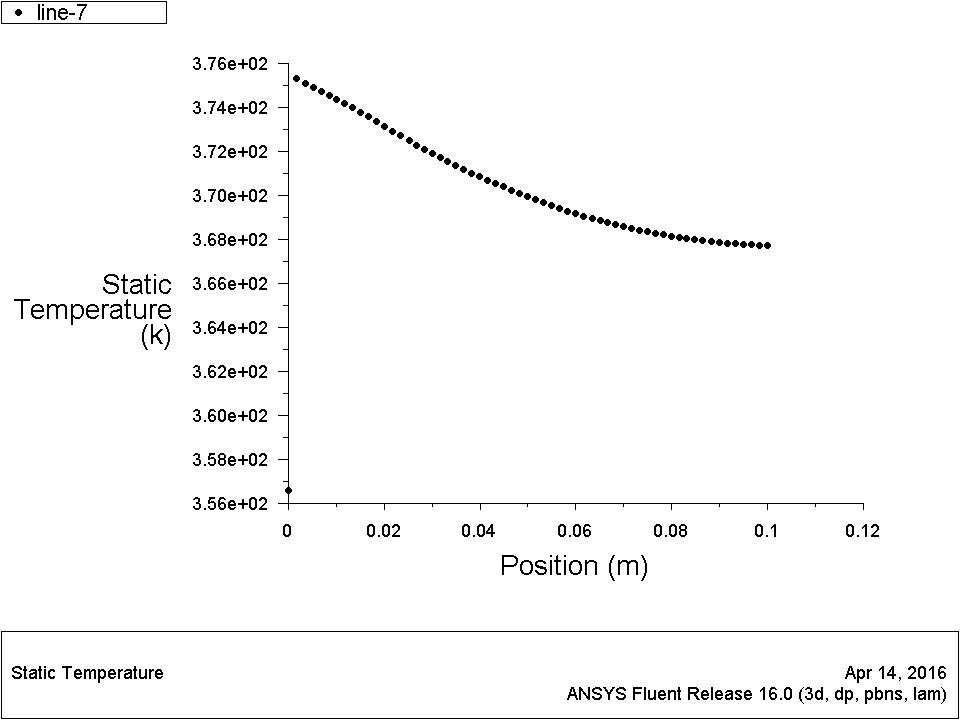
\includegraphics[width=\textwidth]{130.jpg}
 		\caption{20 mm hole}
 		\label{fig:unstructured}
 	\end{subfigure}
 	~ %add desired spacing between images, e. g. ~, \quad, \qquad, \hfill etc.
 	%(or a blank line to force the subfigure onto a new line)
 	\begin{subfigure}[b]{0.5\textwidth}
 		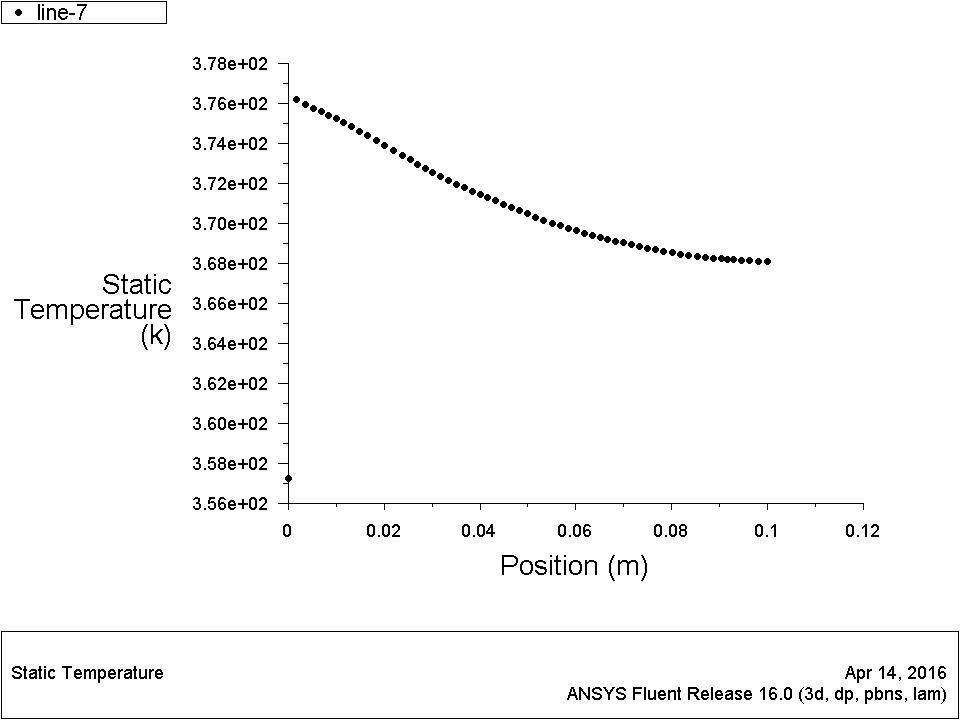
\includegraphics[width=\textwidth]{131.jpg}
 		\caption{23mm hole}
 		\label{fig:structured}
 	\end{subfigure}%
 	~ %add desired spacing between images, e. g. ~, \quad, \qquad, \hfill etc.
 	%(or a blank line to force the subfigure onto a new line)
 	\begin{subfigure}[b]{0.5\textwidth}
 		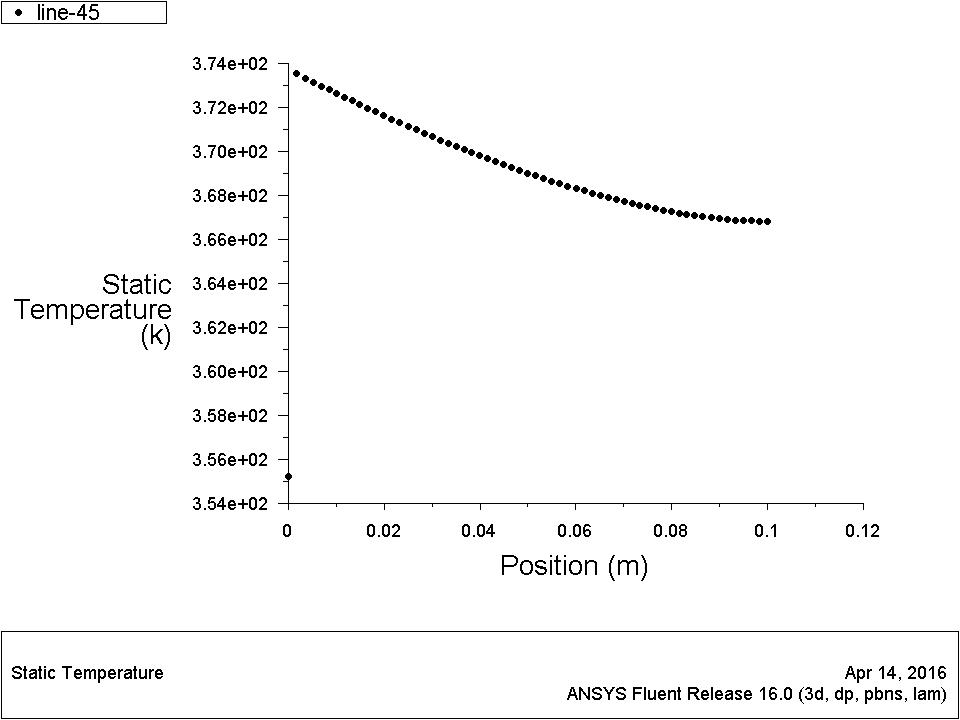
\includegraphics[width=\textwidth]{132.jpg}
 		\caption{variable hole}
 		\label{fig:unstructured}
 	\end{subfigure}

 	~ %add desired spacing between images, e. g. ~, \quad, \qquad, \hfill etc.
 	%(or a blank line to force the subfigure onto a new line)
 	\caption{h variation along length }\label{fig:Meshing}
 \end{figure}
 

\section{Performance Comparison}
The performance of plate fin with different hole diameter is studied, analysed and plotted. The effective heat transfer coefficient for each fin is also found. From these values the percentage Increase of heat transfer coefficient is also found. As the overall heat transfer increases more heat gets dissipated through the fin and hense the base temperature gets reduced. The percentage decrease in base temperature from the plain fin also found and plotted.(table 6.1 and 6.2).

 \begin{table}[h]
 	\centering
 	\begin{tabular}{|l|r|c|}  % use c for center alignment
 		\hline
 		Cases & Base Temperature & \% decrease in $(T_b - T_\infty)$ \\
 		\hline
 		0mm & 385.802 & 28.6 \\
 		5mm & 382.78 & 27.59 \\
 		10mm & 378.08 & 26.02 \\
 		15mm & 375.82 & 25.27 \\
 		20mm & 375.64 & 25.21 \\
 		23mm & 376.53 & 25.51 \\
 		varaible hole & 373.75 & 24.59 \\
 		\hline
 	\end{tabular}
 	\caption{Base Temperature Comparison}
 \end{table}


 \begin{table}[h]
 	\centering
 	\begin{tabular}{|l|c|r|}  % use c for center alignment
 		\hline
 		Cases & $h_{eff} $ & \% inc in $ h_{eff} $ \\
 		\hline
 		5mm & 2.89 & 3.65  \\
 		10mm & 3.07 & 9.88 \\
 		15mm & 3.16 & 13.15 \\
 		20mm & 3.17 & 13.42 \\
 		23mm & 3.13 & 12.11 \\
 		var hole & 3.25 & 16.28 \\
 		\hline
 	\end{tabular}
 	\caption{$h_{eff} $ Comparison}
 \end{table}

\chapter{Conclusion}
The objective of this study were successfully met by computationally simulating the performance of plate fin with and without the presence of holes. The corresponding values of their base temperature and overall heat transfer coefficient were found and compared. Moreover, we noticed that the effect of an alteration of geometric parameters such as position and size of hole influences the other parameters such as temperature profile, base temperature etc.
The performance maps of interesting parameters like the heat transfer coefficient, temperature profile, velocity contour , base temperature variation, effective heat transfer coefficient were also plotted for all confirurations. They can be very useful tools during a design process. The tremendous ability and potential for heat transfer removal, for a plate fin has been pointed out.
An examination of sectioned part of the plate fin was performed, which proved the great contribution that the holes provide in the total heat transfer removal process.

\begin{figure}[h]
	\label{ss}    %Figure Label is used
	\centering
	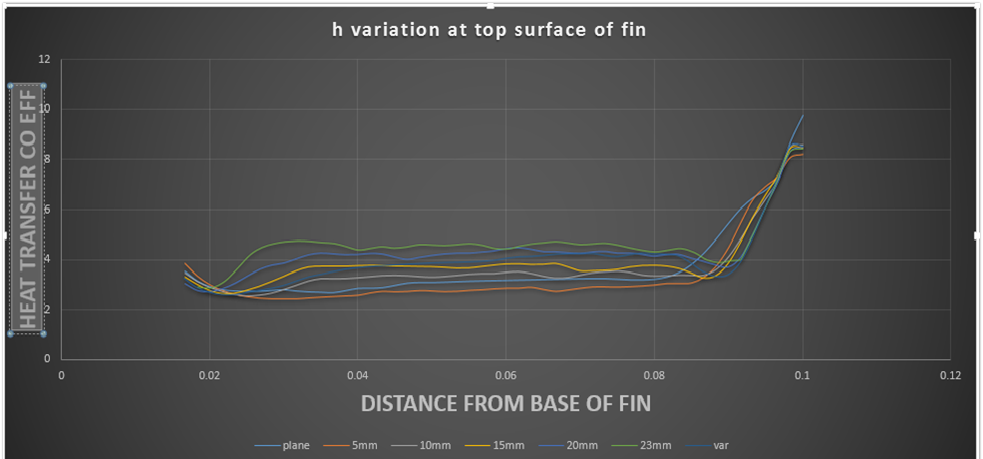
\includegraphics[width= 11 cm]{119.png}
	\caption{$h_{eff}$ Comparison}
\end{figure}

\begin{figure}[h]
	\label{ss}    %Figure Label is used
	\centering
	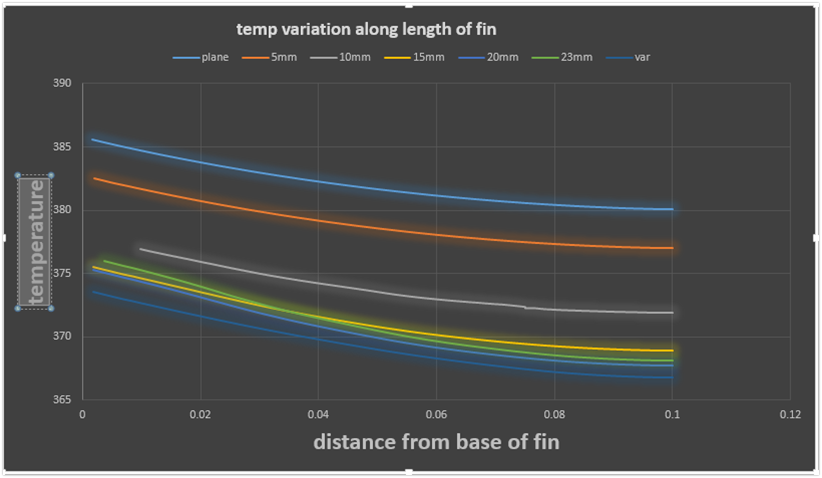
\includegraphics[width= 11 cm]{120.png}
	\caption{Temperature Comparison}
\end{figure}

\begin{figure}[h]
	\label{ss}    %Figure Label is used
	\centering
	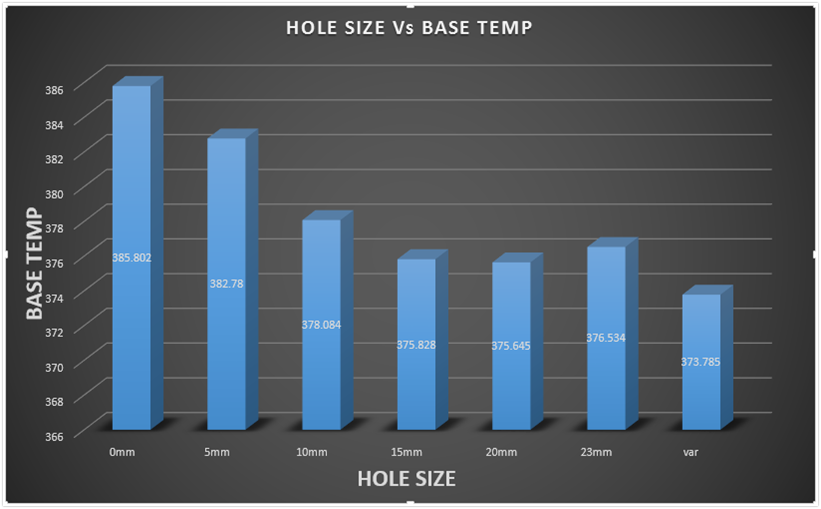
\includegraphics[width= 11 cm]{118.png}
	\caption{Base Temperature Comparion}
\end{figure}



\chapter{Future Scope}

The design of a plate fin for a practical application is thus a complicated process. Many of the approximations cannot be used while designing a actual plate fin.Thus we can improve the experiment accuracy by 

\begin{itemize}
	\item Increasing number of holes \\
	impinging the fin with more finer and smaller hole will provide much satisfactory results.
	\item Viscous dissipation \\
	Likewise to get a more total picture of the performance in future work we
	recommended that the viscous dissipation effects be taken into account in a
	computational model, in order to check how this negatively affects the output.
	\item Shape and Material \\
	Also the examination of configurations with other shape fins that will
	provide better flow characteristics and will be more effective is emerging, while
	the difference on the heat transfer performance that the liquids will provide has to
	be considered.
	\item Forced flow convection
	The experiment can also be extended for analysing forced covection also.
\end{itemize}


%%%%%%%%%%%%%%%%%%%%%%%%%%%%%%%%
%%%%%%%%%%%%%%%%%%%%%%%%%%%%%%%%
%%%%%%%%%%%%%%%%%%%%%%%%%%%%%%%%
\clearpage
%%%%%%%%%%%%%%%%%%%%%%%%%%%%%%%%
%%%%%%%%%%%%%%%%%%%%%%%%%%%%%%%%
%%%%%%%%%%%%%%%%%%%%%%%%%%%%%%%%
%
%                       If u have any Publications Related to this Work
%                 	 If no Publications delete this 
%%%%%%%%%%%%%%%%%%%%%%%%%%%%%%%%

%  \addcontentsline{toc}{chapter}{\quad Publications Related to this Work}
%   \chapter*{\centering{Publications Related to this Work}}

%    \begin{itemize}
%        \item{Presented the paper  in Conference held at VAST, Thrissur, %             March 2013}
%        \item{Paper}

%    \end{itemize}


%%%%%%%%%%%%%%%%%%%%%%%%%%%%%%%%%%%%
%%%%%%%%%%%%%%%%%%%%%%%%%%%%%%%%%%%%
%%
%%          Bibliography 
%%
%%%%%%%%%%%%%%%%%%%%%%%%%%%%%%%%%%%%
%%%%%%%%%%%%%%%%%%%%%%%%%%%%%%%%%%%%

\clearpage
\addcontentsline{toc}{chapter}{\quad Bibliography}
\begin{thebibliography}{99}
%%%%%%%%%%%%%%%%%%%%%%%%%%%%%%%%%%%%
%%
%%          Add Bibliography from below, here 3 eg are there
%%	    If u need to add more bib  use \bibitem   command again & again
%%
%%%%%%%%%%%%%%%%%%%%%%%%%%%%%%%%%%%%

\bibitem{a}
Golnoosh Mostafavi “NATURAL CONVECTIVEHEAT TRANSFER FROM INTRUPTED RECTANGULAR FINS” nov 2012 in university of TEHRAN


\bibitem{b}
HEAT AND MASS TRANSFER by Yunus A Cengel and Afshin J Ghajar 4th edition ,
Tata McGraw Hill Education Private Limited ,NEW DELHI.


\bibitem{c}
Hatada, T., Ueda, U., Oouchi, T. and Shimitz, T. (1989) Improved heat transfer performance of air coolers by strip
fins controlling air flow distribution, ASHRAE Trans., Vol. 95, pp. 166-170.

\bibitem{d}
Beecher, D. T. and Fagan, T. J. (1987) Effect of fin pattern on the air-side heat transfer coefficient in plate finnedtube
heat exchangers, ASHRAE Trans, Vol. 93, pp. 1961-1984.

\bibitem{e}
Patanker, S. V. (1980) Numerical Heat Transfer and Fluid Flow, McGraw-Hill Inc., USA.

\bibitem{f}
Webb, R. L. (1994) Principles of Enhanced Heat Transfer, John Wiley and Sons, USA, pp. 125-127.

\end{thebibliography}



%%%%%%%%%%%%%%%%%%%%%%%%%%%%%%%%%%%%%
%%%%%%%%%%%%%%%%%%%%%%%%%%%%%%%%%%%%%
%\clearpage
%\addcontentsline{toc}{chapter}{\quad APPENDIX}
%\chapter*{\centering{APPENDIX}}
%%%%%%%%%%%%%%%%%%%%%%%%%%%%%%%%%%%%%
%%                          
%%		APPENDIX
%%    if u have pgms make that a pdf & add it here, like the data sheets
%%
%%    If you need to give an Intro to the Appendix
%%                                 Otherwise Delete it . . . 
%%
%%%%%%%%%%%%%%%%%%%%%%%%%%%%%%%%%%%%%
%%%%%%%%%%%%%%%%%%%%%%%%%%%%%%%%%%%%%


% Photovoltaic (PV) power supplied to the system is gaining more and   more  visibility while the demand for power in compared to traditional   energy sources like gas, oil, coal, hydro wind, etc.  .. . \\

% Pgm Code for the IC's\\

% Datasheet of IC's\\

% Datasheet of MOSFETs


%%%%%%%%%%%%%%%%%%%%%%%%%%%%%%%%%%%%%
%%%%%%%%%%%%%%%%%%%%%%%%%%%%%%%%%%%%%
%%                      
%%                      For Adding PDF (Data Sheets) for the Appendix
%%
%%%%%%%%%%%%%%%%%%%%%%%%%%%%%%%%%%%%%
%%%%%%%%%%%%%%%%%%%%%%%%%%%%%%%%%%%%%


% 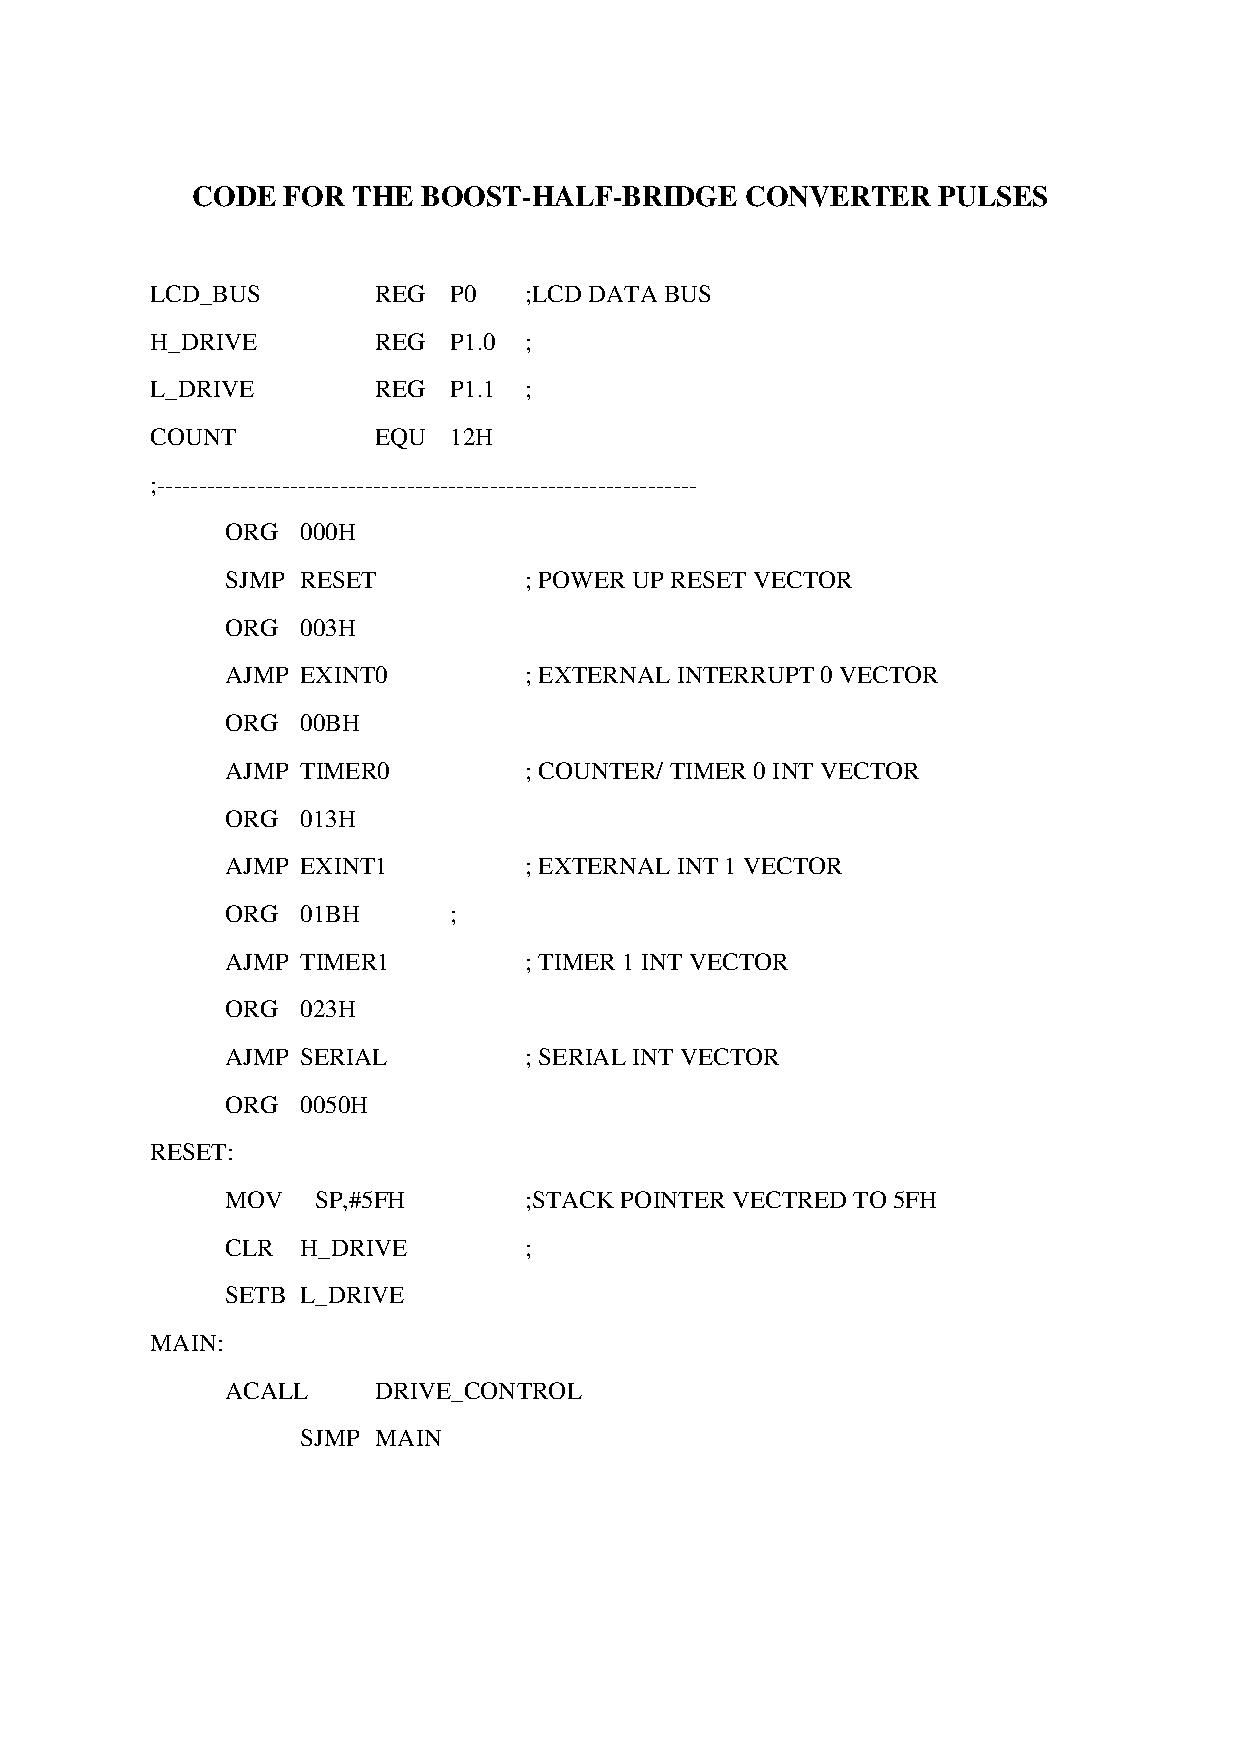
\includepdf[pages=-]{A1.pdf}    % for adding full Paper in PDF
% 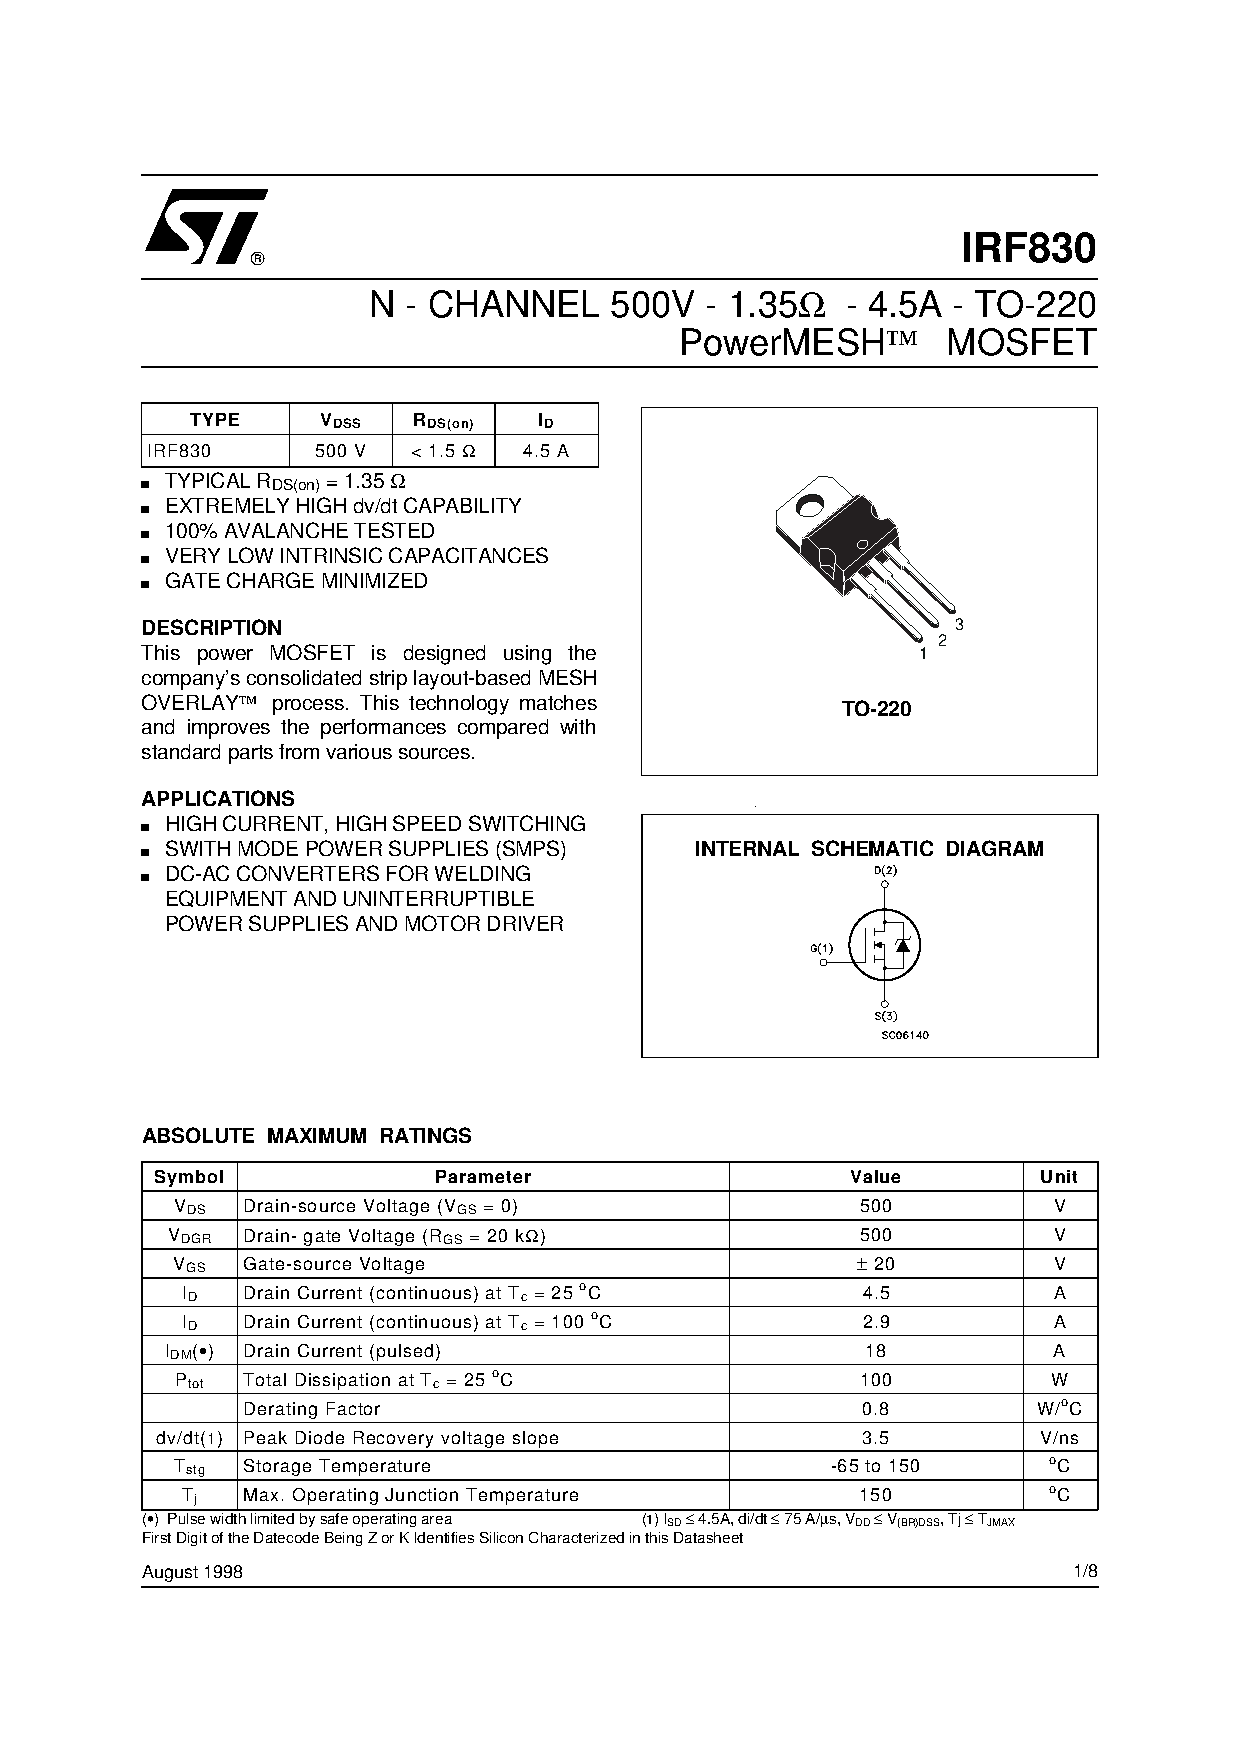
\includepdf[pages=1-3]{IRF830.pdf}    % for adding Pages from 1 to 3 only


%%%%%%%%%%%%%%%%%%%%%%%%%%%%%%%%%%%%%
%%%%%%%%%%%%%%%%%%%%%%%%%%%%%%%%%%%%%
%%%%%%%%%%%%%%%%%%%%%%%%%%%%%%%%%%%%%
%%%%%%%%%%%%%%%%%%%%%%%%%%%%%%%%%%%%%


%%%%%%%%%%%%%%%%%%%%%%%%%%%%%%%%%%%%%
%%%%%%%%%%%%%%%%%%%%%%%%%%%%%%%%%%%%%
%
%   Hi, All
%   Arun Xavier, VAST Thrissur
%
%   for more  Visit my Page - http://arunxeee.blogspot.in/
%
%%%%%%%%%%%%%%%%%%%%%%%%%%%%%%%%%%%%
%%%%%%%%%%%%%%%%%%%%%%%%%%%%%%%%%%%%

%
\end{spacing}
\newpage
\thispagestyle{empty}
\vspace*{\fill}
\begin{flushright}

\includegraphics[width=2.5 cm]{geclogo.png}\\[.2 cm]
{\Large \bf \rm  Department of \vdept\ }\\
{\large \rm Govt Engineering College\\
Sreekrishnapuram , Palakkad - 679 513\\
({\tt http://www.gecskp.ac.in})}
\end{flushright}

%
\end{document}



%%%%%%	Any Problems Contact me  @  arunxeee.blogspot.com
%%%%%									aruncx@gmail.com
%%%%%%%%%%%%%%%%
%%%%
%%%%
%%%%%%%%%%%
%%
%